\chapter{A Dichotomy Theorem for Automatic Structures}

\begin{abstract}
	\marginnote[1.3em]{
		TODO: Section X has been published in BLA.

		Part of the dichotomy theorem---Sections X and Y---was proven during the internship
		of Antoine Cuvelier that I supervised in Summer 2024.

		We thank Joanna Fijalkow for helpful discussions on constraint satisfaction problems.
	}%
	We study the separation problem of "synchronous relations", "aka" "automatic relations",
	by "recognizable relations"---namely finite unions of Cartesian products of "regular languages".
	We prove it to be computationally equivalent to the "finite regular colourability of synchronous graphs", that takes an "rational presentation" of a "graph" as input, and asks whether
	it admits a "regular colouring"---meaning that for each colour, the set of words representing the elements having this colour is a "regular language"---with finitely many colours.

	We first show that, if the number of colours is fixed to be any natural number $k \geq 2$, then
	this problem is undecidable. This implies the undecidability of the separation problem
	of "synchronous relations" by "recognizable relations" where the number of unions allowed is bounded.

	We then generalize this result, and prove a dichotomy theorem for automatic structures:
	for any "relational structure" $\?B$, the problem of whether an "automatic structure"
	admits a "homomorphism" to $\?B$ is either decidable in "NL", or is undecidable.
	We extend these results to "regular homomorphisms", for which we require the "homomorphisms"
	to be "regular@@hom", in the sense that every preimage of any element of the "target structure" $\?B$ must be a "regular language". In both cases, "structures" for which the problem is 
	decidable are those with ``"finite duality"''. 
	
	Using this dichotomy theorem, we then prove that the original problem, 
	namely the separation problem of "synchronous relations"
	by "recognizable relations" is undecidable.
\end{abstract}
\clearpage
\chaptertoc
\clearpage



Let \AP$\intro*\Fin$ denote the class of all "finite $\sigma$-structures",
\AP$\intro*\Aut$ the class of all "automatic $\sigma$-structures".
We let \AP$\intro*\AutPres$ be the class of all "rational presentations of $\sigma$-structures",
and \AP$\intro*\FinPres$ be the subclass of "presentations" of "finite $\sigma$-structures".

We denote by \AP$\intro*\HomFinClass{\?B}$ and $\intro*\HomAllClass{\?B}$ the class
of all finite (resp. all) "$\sigma$-structures" that admit a "homomorphism" to $\?B$.

Given a "$\sigma$-structure" $\?B$, and a class $\classStruct$ of "rational presentations of $\sigma$-structures", we denote by \AP$\intro*\HomDec{\classStruct}{\?B}$ the class of all presentations $\•A \in \classStruct$ such that the "$\sigma$-structure" $\?A$
that they "represent@@structure" admits a "homomorphism" to $\?B$.
Similarly, we denote by \AP$\intro*\HomRegDec{\classStruct}{\?B}$ the class 
associated to "regular homomorphisms".%
\sidenote{Todo: set-theoretic bullshit. Not a set but it is if we fix an alphabet. Blabla.}

While the existence of a "homomorphism" from some "rational presentation" of $\?A$ 
to a "finite $\sigma$-structure" $\?B$ only depends on $\?A$ and not the "presentation" itself,
this is not true for "regular homomorphism".
For a $\sigma$-structure $\?B$,
we use \AP$\intro*\HomFinDec{\?B}$, $\intro*\HomAutDec{\?B}$, $\intro*\HomRegFinDec{\?B}$
and $\intro*\HomRegAutDec{\?B}$ as shorthands for $\HomDec{\FinPres}{\?B}$, $\HomDec{\AutPres}{\?B}$,
$\HomRegDec{\FinPres}{\?B}$ and $\HomRegDec{\AutPres}{\?B}$, respectively.

Note that any "homomorphism" from an "rational presentation" of a "finite structure"
to a "finite structure" is also "regular@@hom" and so $\HomFinDec{\?B} = \HomRegFinDec{\?B}$.\sidenote{Note also that membership in $\HomFinDec{-} = \HomRegFinDec{-}$ and in
$\HomAutDec{-}$ only depends on the "structure represented"
by the "rational presentation", and not on the "presentation" itself.
This is not the case for $\HomRegAutDec{-}$. We use these definitions for two reasons: (1) for consistency with $\HomRegAutDec{-}$ and (2) for the associated decision problem to be defined unambiguously. Note moreover that in the case of "finite structures", the size of its representation, say using adjacency lists, and of its "rational presentation" are equal up to a TODO}

\section{\AP\label{sec:dichotomy-introduction}%
	Introduction}

\begin{theorem}[Dichotomy Theorem for Automatic Structures]
	\!\footnote{The equivalence between (1) and (2) still holds
	when the "homomorphism problem" takes as input ``higher-order automatic
	structures'' as defined in \cite[last remark of \S~XII.3]{Blumensath2024MSOModelTheory},
	since such structures have a decidable first-order theory.}%
	%%%
	\AP\label{thm:dichotomy-theorem-automatic-structures}
	Let $\?B$ be a "finite $\sigma$-structure". The following are equivalent:
	\begin{description}
		\itemAP[\intro*\itemDTFinDual.] $\?B$ has "finite duality";
		\itemAP[\intro*\itemDTHomDec.] $\HomAutDec{\?B}$ is decidable;
		\itemAP[\intro*\itemDTHomRegDec.] $\HomRegAutDec{\?B}$ is decidable;
		\itemAP[\intro*\itemDTEqual.] $\HomAutDec{\?B} = \HomRegAutDec{\?B}$ "ie" for any "automatic presentation" $\•A$ of a 
		"$\sigma$-structure" $\?A$, there is a "homomorphism" from $\?A$ to $\?B$ "iff" 
		there is a "regular homomorphism" from $\•A$ to $\?B$;
		\itemAP[\intro*\itemDTFirstOrder.] $\HomAllClass{\?B}$ has "uniformly first-order definable homomorphisms".
	\end{description}
	Moreover, when $\HomAutDec{\?B}$ and $\HomRegAutDec{\?B}$ undecidable, they are "coRE"-complete
	and "RE"-complete, respectively. When they are decidable, they are TODO.
\end{theorem}
	  
TODO: say that to have "finite duality" can be decided.
\section{Preliminaries}
\label{sec:dichotomy-preliminaries}

\subsection{Regular Homomorphisms}

Given two regular languages $K$ and $L$,%
\footnote{Note that whether $K$ and $L$ share the same alphabet is irrelevant since we can always work on the union of their alphabet.}
a \AP""regular function"" from
$K$ to $L$ is a function $f\colon K \to L$ "st" the relation
\[
	\{\tup{u, f(u)} \mid u \in K\}
\]
is "automatic@@rel".
A \AP""regular homomorphism"" between two "presentations of automatic $\sigma$-structures"
$\•A$ and $\•B$ is a "regular function" from $\domainPres{\•A}$ to $\domainPres{\•B}$
that defines a "homomorphism" from $\?A$ to $\?B$.\footnote{We use the terminology ``regular''
instead of ``automatic'' simply because ``automatic homomorphism'' sounds somewhat weird.}\footnote{Note that "regular homomorphisms" are to "automatic structures" what ``definable homomorphisms''
are to ``definable structures'' in \cite{KlinLasotaOchremiakTorunczyk2016HomomorphismProblems}: they form a restriction on the notion of "homomorphisms" to make then finitely describable---although the "source structure" might be infinite---, using the same logical framework as the one used to describe the "source structure".}%
\footnote{The related notion of ``regular isomorphism''
(under the name ``automatic isomorphism'') was studied in
\cite[Definition~6.10]{KhoussainovNerode1995AutomaticPresentations}. They showed that for any
"$\sigma$-structure" $\?A$,
there are either zero, one, or $\omega$ many "automatic presentations" of $\?A$
up to ``regular isomorphism'' \cite[Theorem~6.8]{KhoussainovNerode1995AutomaticPresentations}.}
We denote by \AP $\•A \intro*\homregto \•B$ the existence of a "regular homomorphism" from
$\•A$ to $\•B$.

\begin{property}
	\label{prop:regular-function-finite-domain}
	Let $f\colon K \to L$ be a function, where $L$ is finite.
	Then $f$ is a "regular function" "iff" for every $v \in L$,
	$f^{-1}[v]$ is a "regular language".
\end{property}

\begin{proof}
	For the left-to-right implication, if $f$ is a "regular function",
	then there exists a first-order formula $\phi(x,y)$ "st"
	for all $\tup{u,v} \in K\times L$, then
	\[
		\univStructSynchronous{\Sigma}, u, v \FOmodels \phi(x,y)
		\text{ "iff" }
		v = f(u).
	\]
	Then given $v\in L$,
	the formula\footnote{``$y = v$'' is not properly defined in the syntax of "first-order logic" but it is straightforward to come up with a formula expressing this property.}
	\[
		\exists y,\, \phi(x,y) \land y = v
	\]
	describes $\{ u\in K \mid f(u) = v \}$, which is hence "regular@@lang".

	Conversely, we consider "first-order formulas" $\phi_{v}$ describing each set
	$\{ u\in K \mid f(u) = v \}$, with $v\in L$. Then
	\[
		\phi(x) \defeq \bigwedge_{v\in L} 
			\phi_{b}(x) \land y = v
	\]
	is a "first-order formula"---since $L$ is finite---describing $f$.
\end{proof}

As a consequence, when $\?B$ is finite, the existence of a "regular homomorphism" to $\?B$
is independent of its "presentation@@auto", and we will hence write $\•A \reintro*\homregto \?B$ 
to mean that $\•A \homregto \•B$.
In particular, a \AP""regular $k$-colouring"" of a "presentation of an automatic graph"
$\•G$ is equivalently a "regular homomorphism" from $\•G$ to $\?K_k$,
or a "$k$-colouring" of $\?G$ "st" for any colour, the set of words of $\domainPres{\•G}$
sharing this colour is a "regular language". 
Unsurprisingly, this property cannot be extended to all "automatic structures":
for instance letting $\+A$ be the "automatic presentation" $\tup{0^*, \set{\tup{0^n,0^{n+1} \mid n \in \N}}}$ of $\tup{\N, \textrm{succ}}$,
and letting $\+A'$ be the "automatic presentation"
$\tup{(00)^*, \set{\tup{0^{2n},0^{2n+2} \mid n \in \N}}}$ of the same "structure",
it can be shown that $\+A \homregto \+A$ but $\+A \nothomregto \+A'$.

\begin{figure}
	\centering
	\begin{tikzpicture}
		\tikzset{every node/.style={fill opacity=.4}}

\node[vertex, draw=c1, fill=c1] at (0,0) (0-0) {};
\foreach \j in {1,...,4} {
	\pgfmathtruncatemacro{\prev}{\j - 1}
	\pgfmathtruncatemacro{\jc}{mod(\j,2) ? 2 : 1}
	\node[vertex, draw=c\jc, fill=c\jc, right=2em of 0-\prev] (0-\j) {};
}
\foreach \i in {1,...,4} {
	\pgfmathtruncatemacro{\prev}{\i - 1}
	\foreach \j in {0,...,4} {
		\pgfmathtruncatemacro{\jc}{mod(\i+\j,2) ? 2 : 1}
		\node[vertex, draw=c\jc, fill=c\jc, above=2em of \prev-\j] (\i-\j) {};
	}
}
\foreach \i in {0,...,4} {
	\node[right=2em of \i-4] (\i-5) {};
}
\foreach \j in {0,...,4} {
	\node[above=2em of 4-\j] (5-\j) {};
}

\foreach \i in {0,...,4} {
	\foreach \j in {0,...,4} {
		\node[below right=-.25em of \i-\j, font=\tiny, color=cDarkGrey] {$x^\j y^\i$};
	}
}

\foreach \i in {0,...,4} {
	\foreach \j in {0,...,4} {
		\draw[edge] (\i-\j) to (\i-\the\numexpr\j+1\relax);
		\draw[edge] (\i-\j) to (\the\numexpr\i+1\relax-\j);
	}
}
	\end{tikzpicture}
	\caption{
		\AP\label{fig:grid-2-reg-colouring}
		A "regular $2$-colouring" of an "automatic presentation" of the infinite quarter-grid.
	}
\end{figure}
In \Cref{fig:grid-2-reg-colouring}, we provide an example of a "regular $2$-colouring":
we let $\+G = \tup{V,\+E}$ be the "automatic presentation" of the infinite quarter-grid,
defined over the alphabet $\{x,y\}$ by $V \defeq x^*y^*$ and
\[
	\+E = \set{\tup{x^p y^q, x^{p+1}y^q} \mid p,q \in \N}
	\cup
	\set{\tup{x^p y^q, x^p y^{q+1}} \mid p,q \in \N}.
\]
Then the unique "$2$-colouring" of $\+G$ assigns one colour%
\footnote{In yellow in \Cref{fig:grid-2-reg-colouring}.} to the
vertices of the form $x^p y^q$ "st" $p-q$ is even.
This "colouring" is of course "regular@@colouring".

Given a fixed "signature" $\sigma$ and a $\sigma$-structure $\?B$,
we denote by:
\begin{itemize}
	\itemAP $\intro*\HomFin{\?B}$ (resp. $\intro*\HomAut{\?B}$, resp.
	$\intro*\HomAll{\?B}$) the class of all "finite $\sigma$-structure"
	(resp. "automatic $\sigma$-structure", resp. arbitrary "$\sigma$-structures")
	that admit a "homomorphism" to $\?B$,
	\itemAP $\intro*\HomRegAut{\?B}$ is the class of all "automatic presentations of  $\sigma$-structures" that admit a "regular homomorphism" to $\?B$.
\end{itemize}
Somewhat abusively, we identify these classes with the associated decision problems---except
for $\HomAll{\?B}$ since arbitrary "$\sigma$-structures" cannot be encoded as finite strings.
For finite structures, we assume the input to be given using adjacency lists, and for "automatic 
structures", we assume the input to be described by an "automatic presentation".
We call $\HomRegAut{\?B}$ the \AP""regular homomorphism problem"" over $\?B$.


\subsection{Constructions on Structures}

Given two "structures" $\?A$ and $\?B$, we define the structure \AP$\intro*\powstruct{\?B}{\?A}$ as follows:
\begin{itemize}
  \item its domain are "homomorphisms" $\?A \to \?B$,
  \item for every "predicate" $\+R$ of arity $k$, for any homomorphism $f_1,\dotsc,f_k$,
  we have $\langle f_1,\dotsc,f_k\rangle \in \+R(\powstruct{\?B}{\?A})$ when 
  \[
	\text{for every }
	\langle a_1,\dotsc,a_k\rangle \in \+R(\?A)
	\text{, we have }
	\langle f_1(a_1), \dotsc, f_k(a_k) \rangle \in \+R(\?B).
  \]
\end{itemize}


\begin{proposition}[Folklore: Currying Homomorphisms]
	\AP\label{prop:currying-hom}
	Given "structures" $\?A$, $\?B$ and $\?C$, if $f\colon \?A\prodstruct \?B \to \?C$
	is a "homomorphism", then $F\colon \?A \to \powstruct{\?C}{\?B}$,
	defined by $a \mapsto (b \mapsto f(a,b))$, is a "homomorphism".
	In fact, this mapping $f \mapsto F$ is a bijection
	between "homomorphisms" $\?A\prodstruct \?B \to \?C$
	and "homomorphisms" $\?A \to \powstruct{\?C}{\?B}$.
\end{proposition}

\begin{proof}
Let $\+R$ be a "predicate" of arity $k$, and let
$\langle a_1,\dotsc,a_k \rangle \in \+R(\?A)$.
We want to show that $\langle F(a_1),\dotsc,F(a_k) \rangle \in \+R(\powstruct{\?C}{\?B})$:
for any $\langle b_1,\dotsc,b_k \rangle \in \+R(\?B)$, we have
\[\langle F(a_1)(b_1), \dotsc, F(a_k)(b_k)\rangle = \langle f(a_1,b_1),\dotsc,f(a_k,b_k) \rangle \in \+R(\?C)\] since $f$ is a "homomorphism" from $\?A\prodstruct \?B$ to $\?C$.
Hence, $F$ is indeed a "homomorphism" from $\?A$ to $\powstruct{\?C}{\?B}$.

Dually, if $F$ is a "homomorphism" from $\?A$ to $\powstruct{\?C}{\?B}$,
we define $f\colon \?A\prodstruct \?B \to \?C$ by $\langle a,b \rangle \mapsto F(a)(b)$,
and claim that $f$ is a "homomorphism". Indeed, if $\+R$ be a predicate of arity $k$,
for any $\langle a_1, \dotsc, a_k \rangle \in \+R(\?A)$
and $\langle b_1, \dotsc, b_k \rangle \in \+R(\?B)$,
we have $\langle f(a_1,b_1), \dotsc, f(a_k,b_k) \rangle
= \langle F(a_1)(b_1), \dotsc, F(a_k)(b_k) \rangle$.
Since $\langle F(a_1), \dotsc, F(a_k) \rangle \in \+R(\powstruct{\?C}{\?B})$
and $\langle b_1, \dotsc,b_k \rangle \in \+R(\?B)$ 
it follows that $\langle F(a_1)(b_1), \dotsc, F(a_k)(b_k) \rangle \in \+R(\?C)$.
Therefore, $f$ is a "homomorphism" from $\?A \prodstruct \?B$ to $\?C$.

It is then routine to check that the maps $f \mapsto F$ and $F \mapsto f$ defined
in the two previous paragraphs are mutually inverse bijections.
\end{proof}

\subsection{Constructions on Automatic Presentations}
\label{sec:construction-automatic-presentations}

Let $\•A$ and $\•B$ be "automatic presentations" of some "$\sigma$-structures"
$\?A$ and $\?B$, over alphabets $\Sigma$ and $\Gamma$, respectively.
We define \AP$\•A \intro*\prodpres \•B$ to be the "presentation@@auto"
over the alphabet $(\Sigma \times \Gamma) \dcup (\Sigma \times \{\pad\}) \dcup (\{\pad\} \times 
\Gamma)$  "st":
\begin{align*}
	\domainPres{\•A\prodpres \•B} & \defeq \{u\convol v \mid u \in \domainPres{\•A} \land v \in \domainPres{\•B}\}\\
	\relPres{\+R}{\•A\prodpres \•B} & \defeq
		\{\tup{u_1\convol v_1,\, \dotsc,\, u_k\convol v_k} \mid
		\tup{u_1,\, \dotsc,\, u_k} \in \relPres{\+R}{\•A} \land
		\tup{v_1,\, \dotsc,\, v_k} \in \relPres{\+R}{\•B}
	\}
\end{align*}
for each "predicate" $\+R$ of arity $k$ in $\sigma$.
It is an "automatic presentation" of $\?A \prodstruct \?B$.
Indeed, given a "first-order formula" $\phi(x_1,\dotsc,x_k)$
over $\signatureSynchronous{\Sigma}$, describing $\relPres{\+R}{\•A}$,
and a "first-order formula" $\psi(x_1,\dotsc,x_k)$
over $\signatureSynchronous{\Sigma}$, describing $\relPres{\+R}{\•B}$,
we let $\phi^*$ (resp. $\psi^*$) be the "formula@@FO" obtained from $\phi$ (resp. $\psi$)
by substituting $\lastLetter{a}(x)$ for $\bigvee_{b \in \Gamma \dcup \{\pad\}} \lastLetter{\tup{a,b}}(x)$ (resp. $\bigvee_{b \in \Sigma \dcup \{\pad\}} \lastLetter{\tup{b,a}}(x)$).
Then $\phi^* \land \psi^*$ is a "first-order formula", over the product alphabet,
that describes $\relPres{\+R}{\•A\prodpres \•B}$. The same construction
works for $\domainPres{\•A\prodpres \•B}$.
This shows that if $\?A$ and $\?B$ are "automatic $\sigma$-structures",
then so is $\?A \times \?B$.\sidenote[][-20em]{Note that the "block product"
is also "automatic@@struct".
For instance, the infinite quarter-grid of \Cref{fig:grid-2-reg-colouring}
can also be constructed as the "block product" of $\tup{\N,+1}$ with itself.}

\begin{proposition}
	\label{prop:homreg-prod-finite}
	Let $\?A$, $\?B$ and $\?C$ be "automatic $\sigma$-structures", such that
	$\?B$ and $\?C$ are finite.
	Let $\•A$ (resp. $\•B$ and $\•B'$, resp. $\•C$ and $\•C'$) be an "automatic presentation"
	of $\?A$ (resp. $\?B$, resp. $\?C$).
	Then $\•A \prodpres \•B \homregto \•C$ "iff" $\•A \prodpres \•B' \homregto \•C'$.
\end{proposition}

\begin{proof}
	The proof follows from the following claim, which can be proven
	exactly in the same fashion as \Cref{prop:regular-function-finite-domain}.

	\begin{claim}
		\label{claim:homreg-prod-finite}
		Assuming again that $\?B$ and $\?C$ are finite,
		a function $f\colon\•A \prodpres \•B \to \•C$ is a "regular homomorphism"
		"iff" for every $b\in \domainPres{\•B}$, for every $c\in \domainPres{\•C}$,
		\(\{
			a\in \domainPres{\•A} \mid f(a,b) = c
		\}\)
		is a "regular language".\qedhere
	\end{claim}
\end{proof}

In other words, the existence of a "regular homomorphism" does not depend on the
"automatic presentation" of the \emph{finite} "structures" that are involved, but only
on the "structure" they represent.
As a consequence of \Cref{prop:homreg-prod-finite}, we write
\(\•A \prodpres \?B \homregto \?C\) as a synonym for \(\•A \prodpres \•B \homregto \•C\).

\begin{corollary}[Currying]
	\label{coro:homreg-currying}
	Let $\?A$, $\?B$ and $\?C$ be "automatic $\sigma$-structures",
	and let $\•A$ be an "automatic presentation" of $\?A$.
	Then $\•A \prodpres \?B \homregto \?C$ "iff" $\•A \homregto \powstruct{\?C}{\?B}$.
\end{corollary}

\begin{proof}
	This also follows from \Cref{claim:homreg-prod-finite}.
\end{proof}

\subsection{Idempotent Core}

\begin{figure}
	\centering
	\begin{tikzpicture}
		\node[vertex, draw=c0, fill=c0, fill opacity=.4] (9) at (0,0) {};
\node[vertex, below right=of 9] (10) {};
\node[vertex, above right=of 10, draw=c1, fill=c1, fill opacity=.4] (11) {};
\node[vertex, below right=of 11] (12) {};
\node[vertex, below right=of 12] (13) {};

% ---
% Transitions
% ---
\foreach \i in {9,11,12} {
	\pgfmathtruncatemacro{\next}{\i + 1}
	\draw[edge] (\i) to (\next);
};
\foreach \i in {10} {
	\pgfmathtruncatemacro{\next}{\i + 1}
	\draw[edge] (\next) to (\i);
}
	\end{tikzpicture}
	\hspace{1cm}
	\begin{tikzpicture}
		\node[vertex] (9) at (0,0) {};
\node[vertex, below right=of 9] (10) {};
\node[vertex, above right=of 10] (11) {};
\node[vertex, below right=of 11] (12) {};
\node[vertex, below right=of 12] (13) {};

\node[vertex, above=of 11, draw=c1, fill=c1, fill opacity=.4] (t2-1) {};
\node[vertex, right=of t2-1, draw=c2, fill=c2, fill opacity=.4] (t2-2) {};
\node[vertex, left=of t2-1, draw=c0, fill=c0, fill opacity=.4] (t2-0) {};

% ---
% Transitions
% ---
\foreach \i in {9,11,12} {
	\pgfmathtruncatemacro{\next}{\i + 1}
	\draw[edge] (\i) to (\next);
};
\foreach \i in {10} {
	\pgfmathtruncatemacro{\next}{\i + 1}
	\draw[edge] (\next) to (\i);
}

\draw[edge] (t2-0) to (t2-1);
\draw[edge] (t2-1) to (t2-2);
\draw[edge] (t2-0) to[bend left=60] (t2-2);

\draw[edge] (9) to[bend left=30] (t2-1);
\draw[edge] (t2-0) to[bend left=30] (11);
\draw[edge] (11) to[bend left=30] (t2-2);
	\end{tikzpicture}
	\caption{\AP\label{fig:dichotomy-idempotent-core}
	Reduction from $\,\HomAll{\marked{\?B}}$ to $\,\HomAll{\?B}$ when $\?B$ 
	is the "$2$-transitive tournament":
	we depict on the left-hand side, the "$\extendedSignature{\sigma}{\?B}$-structure"
	$\?A \not\in \HomAll{\marked{\transitiveTournament{2}}}$,
	and on the right-hand side, the "$\sigma$-structure" $\Phi(\?A)
	\not\in \HomAll{\transitiveTournament{2}}$ to which it is reduced.
	The "interpretation@@predicate" of unary predicates in $\?A$
	are described using colours.}
\end{figure}
We fix a "purely relational signature" $\sigma$.
Given a "$\sigma$-structure" $\?B$,
we denote by \AP$\intro*\extendedSignature{\sigma}{\?B}$
the signature obtained from $\sigma$ by adding
a unary predicate \AP$\intro*\unarypred{b}$ for each $b\in B$.
The \AP""marked structure"" \AP$\intro*\marked{\?B}$ of $\?B$ is the
"$\extendedSignature{\sigma}{\?B}$-structure"
obtained from $\?B$ by "interpreting@@predicate" each predicate $\unarypred{b}$ as the
singleton $\{b\}$.

\begin{proposition}[Folklore]
	\!\sidenote{This reduction is folklore, see "eg"
	\cite[Lemma 2.5]{LaroseTesson2009UniversalAlgebraCSP}.
	We provide here a self-contained proof.}%
	\sidenote{The "marked structure" $\marked{\core{\?B}}$ of the "core" of $\?B$ is
	usually called the \AP""idempotent core""
	of $\?B$. From this proposition, we get that $\HomFin{\?B}$ and
	$\HomFin{\marked{\core{\?B}}}$ are "first-order equivalent".
	This reduction is a central tool
	in the algebraic approach to understand "constraint satisfaction
	problem" since the algebra associated to the "CSP" over an "idempotent core"
	only has idempotent operations, making it much easier to work with.}%
	%%%
	\AP\label{prop:idempotent-core-preserves-csp-complexity}
	If $\?B$ is a finite "core", then the problems $\HomAll{\marked{\?B}}$ and 
	$\HomAll{\?B}$ are "first-order equivalent".
	Moreover, this equivalence preserves "finiteness@@structure",
	in the sense that "finite structures" are mapped to "finite structures".  
	Hence, by restricting this equivalence, we also obtain that
	$\HomFin{\marked{\?B}}$ and $\HomFin{\?B}$ are "first-order equivalent".
\end{proposition}

The non-easy part is to reduce $\HomFin{\marked{\?B}}$ to $\HomFin{\?B}$: only this reduction
requires the assumption that $\?B$ is a core.

\begin{proof}[Proof of \Cref{prop:idempotent-core-preserves-csp-complexity}]
	\proofcase{Reduction from $\,\HomAll{\?B}$ to $\,\HomAll{\marked{\?B}}$.}\\
	We reduce a "$\sigma$-structure" $\?A$ to the
	"$\extendedSignature{\sigma}{\?B}$-structure" $\?A'$ obtained
	from $\?A$ by "interpreting@@predicate" each predicate $\unarypred{b}$ as the empty set.
	Clearly, a function from $A$ to $B$ is a "homomorphism" from $\?A$ to $\?B$
	"iff" it is a "homomorphism" from $\?A'$ to $\marked{\?B}$, proving the correctness
	of the reduction. It is, by definition, "first-order@@reduction".

	\proofcase{Reduction from $\,\HomAll{\marked{\?B}}$ to $\,\HomAll{\?B}$.}
	We first define the reduction $\Phi$ and show its correctness; the fact that it
	is a "first-order reduction" is straightforward.
	We reduce a "$\extendedSignature{\sigma}{\?B}$-structure" $\?A$ to the "$\sigma$-structure"
	$\Phi(\?A)$ illustrated on \Cref{fig:dichotomy-idempotent-core} and defined as follows:
	\begin{itemize}
		\item its underlying universe is the disjoint union $A \dcup B$,
		\item given a "predicate" $\+R$ of arity $k$, its "hyperedges" are:
		\begin{itemize}
		\item all "$\+R$-tuple" of $\?A$,
		\item all "$\+R$-tuple" of $\?B$, and
		\item all "$\+R$-tuple" $\tup{b_1,\dotsc,b_{i-1}, a_i, b_{i+1},\dotsc,b_k}$
			"st" there exists $b_i$ for which the $\+R$-"hyperedge"
			$\tup{b_1,\dotsc,b_{i-1}, b_i, b_{i+1},\dotsc,b_k}$
			is in $\+R(\?B)$, and $a_i$ belongs to the "interpretation@@predicate" of 
			$\unarypred{b_i}$ in $\?A$.
		\end{itemize}
	\end{itemize}
	Note that by construction, the "adjacency" of $a \in A$ in $\Phi(\?A)$ is
	the union of its "adjacency" in $\?A$, and the union of the "adjacencies" of
	$b$ in $\?B$ for all $b$ "st" $a \in \unarypred{b}(\?A)$.

	We show that $\?A \in \HomAll{\marked{\?B}}$ "iff" $\Phi(\?A) \in \HomAll{\?B}$.
	So, assume that there exists a "homomorphism" $f\colon \?A \to \marked{\?B}$.
	Then we let $f'\colon A \dcup B \to B$ be defined by $f'(a) = f(a)$ for all $a\in A$ and
	$f'(b) = b$ for all $b \in B$. We claim that $f'$ is a "homomorphism" from
	$\Phi(\?A)$ to $\?B$. Indeed, consider a "hyperedge" of $\Phi(\?A)$:
	\begin{itemize}
		\item if it is a "hyperedge" of $\?A$, its image by $f'$ is still a "hyperedge"
			of $\?B$ since $f$ is a "homomorphism" from $\?A$ to $\marked{\?B}$;
		\item if it is a "hyperedge" of $\?B$, then its image by $f'$ is itself, and is hence
			a "hyperedge" of $\?B$;
		\item otherwise, it must be of the form 
			\[\tup{b_1,\dotsc,b_{i-1}, a_i, b_{i+1},\dotsc,b_k}\]
			"st" there exists $b_i$ for which
			$\tup{b_1,\dotsc,b_{i-1}, b_i, b_{i+1},\dotsc,b_k} \in \+R(\?B)$
			and $a_i \in \unarypred{b_i}(\?A)$:
			in this case, its image by $f'$ is 
			\[f'(\tup{b_1,\dotsc,b_{i-1}, a_i, b_{i+1},\dotsc,b_k})
			= \tup{b_1,\dotsc,b_{i-1}, b_i, b_{i+1},\dotsc,b_k} \in \+R(\?B)\]
			since $f'(b) = b$ for all $b\in B$ and $f'(a_i) = f(a_i) = b_i$ since
			$a_i \in \unarypred{b_i}(\?A)$ and $f$ is a "homomorphism" from
			$\?A$ to $\marked{\?B}$.
	\end{itemize}
	And hence, $\Phi(\?A) \homto \?B$.

	Conversely, now let $g\colon \Phi(\?A) \to \?B$ be a "homomorphism".
	Its restriction to $\?B$, namely $\restr{g}{B}$ is a "homomorphism" from $\?B$
	to itself, and since $\?B$ is a "core", it must be an "automorphism" over $\?B$
	by \Cref{prop:core-iff-hom-are-auto}.
	We then define a map $g' \colon A \to B$ by sending
	$a$ to $(\restr{g}{B})^{-1}\circ g(a)$, and claim that it is a "homomorphism"
	from $\?A$ to $\marked{\?B}$. As a matter of fact, it clearly preserves "$\+R$-tuple"
	for any $\+R$ in $\sigma$, since $g$ and $(\restr{g}{B})^{-1}$ are "homomorphisms".
	We must then show that it preserves all unary "predicates" $\unarypred{b}$, with $b\in B$:
	let $a \in A$ "st" $\unarypred{b}$ holds, "ie" $a \in \unarypred{b}(\?A)$.
	Now, by construction of $\Phi(\?A)$, the "adjacency" of $g(a)$ in $\?B$
	and the "adjacency" of $g(b)$ in $\?B$ are equal.
	Since $\?B$ is a "core", it follows by \Cref{prop:adjacency-core} that $g(a) = g(b)$.
	By definition of $g'$, this rewrites as $g'(a) = b$, "ie" $g'(a) = \unarypred{b}(\marked{\?B})$.
	Therefore, we have built a "homomorphism" from $\?A$ to $\marked{\?B}$.

	Overall, this proves that $\Phi$ is correct.
	It is trivially a "first-order reduction" and moreover,
	it preserves "finiteness@@structure" since $\?B$
	is "finite@@structure".
\end{proof}


\subsection{De Bruijn–Erdős Theorem}

\begin{proposition}[""De Bruijn–Erdős Theorem""]
	\!\footnote{It is straightforward to note that
	one can replace ``every finite "substructure"'' by
	``every finite "induced substructure"'' in the statement of the theorem.
	The original theorem is about graph colouring, but the generalization is straightforward.}%
	\AP\label{prop:de-bruijn-erdos}
	Let $\?A$ be an arbitrary "$\sigma$-structure" and $\?B$ a "finite $\sigma$-structure".
	There is a "homomorphism" from $\?A$ to $\?B$ "iff" for every finite "substructure" $\?A'$
	of $\?A$, there is a "homomorphism" from $\?A$ to $\?B$.
\end{proposition}

\begin{proof}
	The left-to-right implication is direct.
	We prove the converse by using the "Tychonoff's compactness theorem".\footnote{This is a direct adaptation from \cite[\S~``Proof'']{Wikipedia2024DeBruijnErdos}.}
	So, assume that for every finite "substructure" $\?A'$ of $\?A$,
	there is a "homomorphism" from $\?A$ to $\?B$. 
	Consider the topological space $B^A$, consisting of all functions from $A$ to $B$,
	together with the product topology.\footnote{We equip $B$ with the discrete topology,
	making it compact since $B$ is finite.} By "Tychonoff's compactness theorem",
	$B^A$ is compact. For each finite subset $X$ of $A$, let
	$H_X$ denote the set of all $f \in B^A$ "st" $\restr{f}{X}$ is a "homomorphism"
	from the "substructure" of $\?A$ "induced@@structure" by $X$ to $\?B$.
	Then, each $H_X$ is closed---indeed, whether $f\in B^A$ belongs to $H_X$ only depends
	on finitely many $f(x)$'s---, and moreover the intersection of finitely many
	$H_X$'s, say $H_{X_1} \cap \cdots \cap H_{X_n}$, is non-empty since
	$H_{X_1} \cap \cdots \cap H_{X_n} \supseteq H_{X_1\cup \dotsc \cup X_n}$
	and by assumption $H_{X_1\cup \dotsc \cup X_n}$ is non-empty since $X_1 \cup \cdots \cup X_n$ is finite. Hence, by compactness of $B^A$ and the "finite intersection property", it follows
	that $\bigcap_X H_X$ is non-empty, which means that there is a "homomorphism" from $\?A$ to $\?B$.
\end{proof}

\begin{corollary}
	\!\footnote{Another important consequence of the "De Bruijn–Erdős Theorem" is that,
	for instance, the notion of "dual" does not depend on whether we are considering finite or
	arbitrary "$\sigma$-structures".}
	\AP\label{coro:de-bruijn-erdos}
	Given arbitrary $\sigma$-structures $\?B_1$ and $\?B_2$, the following are equivalent:
	\begin{enumerate}
		\itemAP\label{item:de-bruijn-erdos-finite} for every finite "$\sigma$-structure" $\?A$, we have $\?A \homto \?B_1$
		"iff" $\?A \homto \?B_2$;
		\itemAP\label{item:de-bruijn-erdos-arbitrary} for every arbitrary "$\sigma$-structure" $\?A$, we have $\?A \homto \?B_1$
			"iff" $\?A \homto \?B_2$;
		\itemAP\label{item:de-bruijn-erdos-hom} $\?B_1$ and $\?B_2$ are "homomorphically equivalent".
	\end{enumerate}
\end{corollary}
\begin{proof}
	\eqref{item:de-bruijn-erdos-arbitrary} $\Rightarrow$ \eqref{item:de-bruijn-erdos-hom}
	and \eqref{item:de-bruijn-erdos-hom} $\Rightarrow$ \eqref{item:de-bruijn-erdos-finite}
	are trivial.
	For \eqref{item:de-bruijn-erdos-finite} $\Rightarrow$ \eqref{item:de-bruijn-erdos-arbitrary},
	we assume "wlog" by contradiction that there is an arbitrary "$\sigma$-structure" $\?A$ "st" $\?A \homto \?B_1$ but $\?A \nothomto \?B_2$. Then by \Cref{prop:de-bruijn-erdos},
	there exists a finite "substructure" $\?A_0$ of $\?A$ "st" $\?A_0 \nothomto \?B_2$.
	But then $\?A_0 \homto \?A \homto \?B_1$, which contradicts \eqref{item:de-bruijn-erdos-finite}.
\end{proof}


\subsection{Obstructions and Finite Duality}

Let $\?B$ and $\?D$ be "finite $\sigma$-structures".
We say that $\?D$ is an \AP""obstruction"" of $\?B$ when $\?D \nothomto \?B$.
In this case, note that finding $\?D$ inside $\?A$---in the sense that $\?D \homto \?A$---implies that $\?A$ cannot have a "homomorphism" to $\?B$: in this sense, the presence of
$\?D$ in an \emph{obstruction} to the existence of a "homomorphism" to $\?B$.

A \AP""dual"" of $\?B$ is any arbitrary set $\+D$ of "finite $\sigma$-structures" "st"
for any "finite $\sigma$-structure" $\?A$:
\[
	\?A \homto \?B
	\text{ "iff" }
	\forall \?D \in \+D,\, \?D \nothomto \?A.
\]
Note that any "dual" must only contain "obstructions" of $\?B$.%
\sidenote[][-20em]{The notion of dual was implicitly introduced
by Ne\v{s}et\v{r}il and Pultr, who proved that for "\emph{undirected} graph", no
non-trivial "finite duality" existed, in the sense that the
only "cores" $\?B$ having a finite "dual" where the empty graph, and the graph having
a single vertex and no edge \cite[Corollary 4.1]{NesetrilPultr1978Duality}.}
The set of all "obstructions" of $\?B$ is a "dual" of $\?B$.

\begin{example}
	\AP\label{ex:dual-T2} Let $k\in\N$. The set
	$\{\pathGraph{k+1}\}$ is a "dual" of the
	"$k$-transitive tournament" $\transitiveTournament{k}$---see \Cref{fig:T2-P2}.
	
	Indeed, $\pathGraph{k+1} \nothomto \transitiveTournament{k}$. Dually,
	if $\?G$ if a "finite graph" "st" $\?G \homto \transitiveTournament{k}$ then
	letting $f$ be a "homomorphism" from $\?G$ to $\transitiveTournament{k}$,
	we have that any edge from $u \in G$ to $v \in G$, we must have $f(u) < f(v)$,
	and so $\pathGraph{k} \nothomto \?G$.
\end{example}

Moreover, if $\+D$ and $\+D'$ are sets of "obstructions" of $\?B$ and $\+D \subseteq \+D'$,
then if $\+D$ is a "dual", so is $\+D'$: hence, the goal is to find \emph{small} duals.
For this reason, "duals" are also called \emph{complete sets of obstructions}.
We say that $\?B$ has \AP""finite duality"" if is admits a finite "dual", "ie"
consisting of finitely many "structures". For instance, $\transitiveTournament{k}$ has "finite duality".

An "obstruction" $\?D$ of $\?B$ is \AP""critical@@obs""\footnote{We borrow the terminology
from \cite{LaroseLotenTardif2007CharacterisationFOCSP}.} when for every
"proper substructure" $\?D'$ of $\?D$, we have $\?D' \homto \?B$.
Clearly, every "critical obstruction" must be a "core".

Note first that the set of all "critical obstructions" of $\?B$ is a "dual" of $\?B$.
Indeed, if $\?A \nothomto \?B$, then $\?A$ is an "obstruction" and so it must contain---by well-foundedness of $\N$---a "critical obstruction" $\?D$ as a "substructure".

\begin{proposition}
	\label{prop:finite-duality-iff-critical-obstructions}
	Let $\?B$ be a "finite $\sigma$-structure". $\?B$ has "finite duality"
	"iff" it has finitely many "critical obstructions".
\end{proposition}

\begin{proof}
	The right-to-left implication is trivial. For the converse one,
	let $\+D = \{D_1,\dotsc,D_m\}$ be a finite "dual" of $\?B$.
	If $\?C$ is a "critical obstruction" of $\?B$ then in particular $\?C \nothomto \?B$
	and so there exists $i \in \intInt{1,m}$ "st" there is a "homomorphism" $f$ 
	from $\?D_i$ to $\?C$. Now the image of $f$ is again an "obstruction" of $\?B$,
	and since $\?C$ is "critical@@obs", it follows that it must be $\?C$ itself. In other
	words, $f$ is "strong onto". In particular, we obtain that $\?C$ is a "quotient@@struct" of
	$\?D_i$. Hence, there are only finitely many "critical obstructions" of $\?B$.
\end{proof}

One of the key interest of \Cref{prop:finite-duality-iff-critical-obstructions} is
to prove that some structures don't have "finite duality".

\begin{figure}
	\centering
	\begin{tikzpicture}
		\node[vertex] (0) at (0,0) {};
\node[vertex, below right=of 0] (1) {};
\foreach \i in {1, 3, 5, 7, 9} {
	\pgfmathtruncatemacro{\next}{\i + 1}
	\pgfmathtruncatemacro{\nnext}{\i + 2}
	\node[vertex, below right=of \i] (\next) {};
	\node[vertex, above right=of \next] (\nnext) {};
};
\node[vertex, below right=of 11] (12) {};
\node[vertex, below right=of 12] (13) {};

% ---
% Transitions
% ---
\foreach \i in {0,1,3,5,7,9,11,12} {
	\pgfmathtruncatemacro{\next}{\i + 1}
	\draw[edge] (\i) to (\next);
};
\foreach \i in {2,4,6,8,10} {
	\pgfmathtruncatemacro{\next}{\i + 1}
	\draw[edge] (\next) to (\i);
}
		
\foreach \i in {1,3,5,7,9,11} {
	\pgfmathtruncatemacro{\half}{\i / 2}
	\node[draw=none, above right=-.6em of \i] {$a_{\half}$};
};
\foreach \i in {2,4,6, 8, 10, 12} {
	\pgfmathtruncatemacro{\half}{(\i / 2) - 1}
	\node[draw=none, below left=-.6em of \i] {$b_{\half}$};
};
\node[draw=none, below left=-.6em of 0] {$a'_0$};
\node[draw=none, above right=-.6em of 13] {$b'_5$};

\draw[decoration={brace}, decorate, transform canvas={yshift=1.5em}] (3.north west) to node[midway, above] {$\+O(n)$ nodes} (11.north east);
	\end{tikzpicture}
	\caption{\AP\label{fig:zigzag-graph}The "zigzag graph" $\zigzag{5}{2}$.}
\end{figure}
\begin{example}[{\Cref{ex:dual-T2}, continued.}]
	\AP\label{ex:zigzag-defn}
	Let $n\in\?N$.
	We define the \AP""zigzag graph"" $\intro*\zigzag{n}{2}$ of width $n$ and length 2
	to be "graph@@dir" whose vertices are $a_0, \dotsc, a_n$, $b_0, \dotsc, b_{n}$,
	$a'_0$ and $b'_n$, with edges from $a_i$ to $b_{i-1}$ and to $b_{i}$ (for $i \in \intInt{0,n}$, whenever the nodes exist), and with an edge from $a'_0$ to $a_0$ and from $b_n$
	to $b'_n$. See \Cref{fig:zigzag-graph} for an illustration.
	
	Note that $\zigzag{n}{2}$ does not admit a "homomorphism" to the "$2$-path"---indeed, such a homomorphism should send $a'_0$, $a_0$ and $b_0$ onto $0$, $1$, and $2$, respectively, 
	and so all $a_i$'s (resp. $b_i$'s) must be sent onto $1$ (resp. $2$), but then $b'_n$ cannot be mapped anywhere.

	We claim that each $\zigzag{n}{2}$ ($n\in\N$) is a "critical obstruction" of $\pathGraph{2}$.
	We have already seen that $\zigzag{n}{2}$ is an "obstruction" of $\pathGraph{2}$.
	But then notice that to obtain a "proper substructure" of $\zigzag{n}{2}$,
	we must either:
	\begin{itemize}
		\item remove the edge from $a'_0$ to $a_0$ or the edge from $b_n$ to $b'_n$,
		in which case it admits a "homomorphism" to $\pathGraph{2}$, or
		\item remove any other edge, in which case the resulting "substructure" is not "connected",
		and both parts admit a "homomorphism" to $\pathGraph{2}$.
	\end{itemize}
	And hence, by \Cref{prop:finite-duality-iff-critical-obstructions}, it follows that
	$\pathGraph{2}$ does not have "finite duality".

	On the other hand, each $\zigzag{n}{2}$ with $n\in\Np$ admits a "homomorphism" to the "$2$-transitive tournament", as witnessed by \Cref{fig:zigzag-graph-hom-T2}.%
	\sidenote[][-11em]{However, observe that $\zigzag{0}{2} = \pathGraph{3}$ is an "obstruction" of
	$\transitiveTournament{2}$.}
	In fact, this "homomorphism" is far from being unique:
	each vertex $a_1,\,a_2,\,\dotsc,\,a_{n-1}$ can be sent on either $0$ or $1$
	(the red and yellow vertices), 
	and similarly, each vertex $b_1,\,b_2,\,\dotsc,\,b_{n-1}$ can be sent on either $1$ or $2$
	(the yellow and blue vertices).%
	\sidenote[][-11em]{
		Note that it is straightforward to extend the fact that
		\[\zigzag{n}{2} \homto \transitiveTournament{2}
		\text{ and }
		\zigzag{n}{2} \nothomto \pathGraph{2}\]
		to arbitrary values of $k\in \N$, in the sense that
		\[\zigzag{n}{k} \homto \transitiveTournament{k}
		\text{ and }
		\zigzag{n}{k} \nothomto \pathGraph{k},\]
		by letting
		$\zigzag{n}{k}$ be the graph obtained from $\zigzag{n}{2}$ by
		replacing the path leading to $a_0$ by a path of length $k-1$.
	}
	\begin{figure}
		\centering 
		\begin{tikzpicture}
			\node[vertex, draw=c0, fill=c0, fill opacity=.4] (0) at (0,0) {};
\node[vertex, below right=of 0, draw=c1, fill=c1, fill opacity=.4] (1) {};
\foreach \i in {1, 3, 5, 7, 9} {
	\pgfmathtruncatemacro{\next}{\i + 1}
	\pgfmathtruncatemacro{\nnext}{\i + 2}
	\node[vertex, below right=of \i, draw=c2, fill=c2, fill opacity=.4] (\next) {};
	\node[vertex, above right=of \next, draw=c0, fill=c0, fill opacity=.4] (\nnext) {};
};
\node[vertex, below right=of 11, draw=c1, fill=c1, fill opacity=.4] (12) {};
\node[vertex, below right=of 12, draw=c2, fill=c2, fill opacity=.4] (13) {};

% ---
% Transitions
% ---
\foreach \i in {0,1,3,5,7,9,11,12} {
	\pgfmathtruncatemacro{\next}{\i + 1}
	\draw[edge] (\i) to (\next);
};
\foreach \i in {2,4,6,8,10} {
	\pgfmathtruncatemacro{\next}{\i + 1}
	\draw[edge] (\next) to (\i);
}

% ---
% 2-transitive tournament
% ---
\node[vertex, above right=-.25em and 5em of 13, draw=c2, fill=c2, fill opacity=.4] (t2-2) {};
\node[vertex, above=of t2-2, draw=c1, fill=c1, fill opacity=.4] (t2-1) {};
\node[vertex, above=of t2-1, draw=c0, fill=c0, fill opacity=.4] (t2-0) {};

\draw[edge] (t2-0) to (t2-1) to (t2-2);
\draw[edge] (t2-0) to[bend left=60] (t2-2);
		\end{tikzpicture}
		\caption{\AP\label{fig:zigzag-graph-hom-T2}A "homomorphism" from the "zigzag graph" (left-hand side) to the "$2$-transitive tournament" (right-hand side).}
	\end{figure}
\end{example}

While $\pathGraph{k}$ and $\transitiveTournament{k}$ are similar structures,
one has "finite duality" and the other does not.

Recall that by "Atserias' theorem", this implies that
$\HomFin{\transitiveTournament{k}}$ is "first-order definable"\footnote{By the formula saying that
there are no variables $x_0$, $\dotsc$, $x_{k+1}$ "st" for all $i$ there is an edge from $x_i$ to $x_{i+1}$.} but $\HomFin{\pathGraph{k}}$ is not.%
\footnote{This can also be proven by hand: for 
instance we let $\tilde{\?Z}^{(n)}_2$ be defined analogously to $\zigzag{n}{2}$ except
that we remove the edge from $a_{k}$ to $b_k$ for $k = \lceil \frac{n}{2} \rceil$. 
Then for a well-chosen single-exponential function $f\colon \N \to \N$, for $n\in\N$,
we have that Duplicator wins the Ehrenfeucht-Fraïssé game on $\zigzag{f(n)}{2}$ and
$\tilde{\?Z}^{(f(n))}_2$. Since $\zigzag{f(n)}{2} \nothomto \pathGraph{2}$ but
$\tilde{\?Z}^{(n)}_2 \homto \pathGraph{2}$, this implies that $\HomFin{\pathGraph{2}}$ is not 
"first-order definable". See "eg" \cite[\S~3]{Kolaitis2007FiniteModelTheory} for details on
Ehrenfeucht-Fraïssé games.}


\begin{remark}[From finite to infinite structures]
	In the property
	\[
		\?A \homto \?B
		\;\text{ "iff" }\;
		\forall \?D \in \+D,\, \?D \nothomto \?A
	\]
	defining a "dual", we quantified $\?A$ over "finite $\sigma$-structures". 
	We could equally quantify over all "$\sigma$-structures" without changing the notion of "dual" by "De Bruijn-Erdős theorem".
\end{remark}

We say that a "$\sigma$-structure" is \AP""rigid"" if its only "automorphism"
is the identity.
\begin{proposition}[{\cite[Lemma~4.1]{LaroseLotenTardif2007CharacterisationFOCSP}}]
	\!\footnote{In fact
	only assumes that $\?B$ has "tree duality": as we will see in 
	\Cref{prop:finite-duality-implies-tree-duality}, this is a weaker condition
	than having "finite duality".}%
	\label{prop:finite-duality-implies-rigid}
	If a finite "core" has "finite duality", then it is "rigid".
\end{proposition}

\subsection{Trees and Tree Duality}

A "$\sigma$-structure" is \AP""strongly acyclic@@struct"" if its "incidence graph" is acyclic.
A \AP""$\sigma$-tree"" is a "$\sigma$-structure" that is both "connected" and "strongly acyclic@@struct".
Do not confuse this notion with the classical notion of "directed trees":
every "directed tree" is a "$\sigma$-tree" for the "graph signature" $\sigma$,
but $\zigzag{n}{2}$---see \Cref{fig:zigzag-graph}---is a "$\sigma$-tree"
while it is not a "directed tree". 

Given a "$\sigma$-tree" $\?T$ and a vertex $t\in T$, the \AP""height@@struct"" of $\?T$
when rooted at $t$ is the maximal "distance@@struct" between $t$ and any other vertex of $\?T$.

We say that a finite "$\sigma$-structure" $\?B$ has \AP""tree duality""
if it admits a (potentially infinite) "dual" consisting only of "$\sigma$-trees".
Somewhat surprisingly, Ne\v{s}et\v{r}il and Tardif showed that
this notion generalizes "finite duality".

\begin{proposition}[{\cite[Theorem~3.1]{NesetrilTardif2000DualityTheorems}}]
	\!\footnote{The statement of \cite[Theorem~3.1]{NesetrilTardif2000DualityTheorems}
	is somewhat cryptic: the relationship with "duals" is given by
	\cite[Lemma~2.5]{NesetrilTardif2000DualityTheorems}.
	We refer the reader to Foniok's Ph.D. for statements that use a terminology closer to ours:
	\cite[Theorem~2.1.12]{Foniok2007PhD} shows that if $\{\?A\}$ is a "dual" of $\?B$,
	then $\?A$ is "homomorphically equivalent" to a tree, "ie" if a "structure" has
	``singleton duality'', then it has "tree duality".
	The generalization to "finite duality" then follows from
	\cite[Theorem~2.4.4]{Foniok2007PhD}.}
	\AP\label{prop:finite-duality-implies-tree-duality}
	If a finite "$\sigma$-structure" $\?B$ has "finite duality",
	then it has "tree duality".
\end{proposition}

The converse does not hold.
\begin{proposition}
	\AP\label{prop:2-path-tree-duality}
	The "$2$-path" $\pathGraph{2}$ has "tree duality".
\end{proposition}

\begin{proof}[Proof sketch]
	It can be shown that $\{\zigzag{n} \mid n\in\N\}$ is a "dual" of
	$\pathGraph{2}$. Moreover, each $\zigzag{n}{2}$ ($n\in\N$) is a "$\sigma$-tree".
\end{proof}

Feder and Vardi introduced a construction to decide if a "finite structure" has "tree duality":
given a "$\sigma$-structure" $\?B$, we let \AP$\intro*\FederVardi{\?B}$ be
the $\sigma$-structure whose domain is $\psetp{B}$, and for every $\+R_{(k)} \in \sigma$,
we have $\tup{Y_1, \dotsc, Y_k} \in \+R(\FederVardi{\?B})$ 
(with $Y_1, \dotsc, Y_k \in \psetp{B}$) precisely when 
for every $i\in \intInt{1,k}$, 
for every $b_i \in Y_i$,
there exists $b_j \in Y_j$ for every $j \neq i$ "st" 
$\tup{y_1, \dotsc, y_k} \in \+R(\?B)$.%
\footnote{In fact $\FederVardi{-}$ can
easily be extended to be a functor in the category of $\sigma$-structures, see
"eg" \cite[\S~9.2.2]{NesetrilPOM2012FirstOrderCSPs}.}
In the case of "graphs@@dir", the nodes of $\FederVardi{\?H}$ are non-empty
subsets of vertices of $\?H$, and there is an edge from $X$ to $Y$ when:
\begin{itemize}
	\item for every $x \in X$, there exists $y\in Y$ "st" $\tup{x,y}$ is an edge of $\?H$, and
	\item for every $y\in Y$, there exists $x\in X$ "st" $\tup{x,y}$ is an edge of $\?H$.
\end{itemize}

By construction, note that $b \mapsto \set{B}$ defines a "homomorphism" from
$\?B$ to $\FederVardi{\?B}$.

\begin{proposition}[{\cite[Theorem 21]{FederVardi1998ComputationalStructure}}]
	\label{prop:charac-Feder-Vardi}
	A "finite $\sigma$-structure" $\?B$ has "tree duality" if, and only if,
	$\FederVardi{\?B} \homto \?B$, or, equivalently, if $\?B$ and $\FederVardi{\?B}$
	are "homomorphically equivalent".
\end{proposition}

Note that $\FederVardi{\FederVardi{\?B}}$ is always "homomorphically equivalent" to
$\FederVardi{\?B}$---see "eg" \cite[\S~9.2.2, Proposition 9.1]{NesetrilPOM2012FirstOrderCSPs}---
and so $\FederVardi{\?B}$ \emph{always} has "tree duality", no matter if $\?B$ has this property.

\begin{example}[{\Cref{ex:zigzag-defn}, continued}]
	\label{ex:Feder-Vardi-P2}
	Using \Cref{prop:charac-Feder-Vardi}, we can prove for instance that
	if a "graph@@dir" $\?G$ has "tree duality", then either it is a "DAG", or $\?G$ contains
	a self-loop.

	Indeed, let $v_0 \to v_1 \to \cdots \to v_m$ be a "directed cycle" in $\?G$,
	with $v_0 = v_m$. Then in $\FederVardi{\?G}$, there is an edge from
	$\{v_0,v_1,\dotsc,v_m\}$ to itself.
	Since $\?G$ has "tree duality", it follows by \Cref{prop:charac-Feder-Vardi}
	that $\FederVardi{\?G} \homto \?G$ and hence $\?G$ also contains a self-loop.
	
	Note that, if $\?G$ contains a self-loop, then actually it is "homomorphically equivalent" to the graph consisting of a single self-loop---that admits $\emptyset$ as a "dual" and hence has
	"tree duality". In other words, what we showed can be rephrased as: any
	non-trivial "graph@@dir" with "tree duality" is a "DAG".
	For instance, this implies that $\clique{2}$ does not have
	"tree duality".
	
	\begin{marginfigure}[-20em]
		\centering
		\begin{tikzpicture}
			% ---
% 2-path graph
% ---
\node[vertex, draw=c2, fill=c2, fill opacity=.4] at (0,0) (p2-2) {};
\node[vertex, above=of p2-2, draw=c1, fill=c1, fill opacity=.4] (p2-1) {};
\node[vertex, above=of p2-1, draw=c0, fill=c0, fill opacity=.4] (p2-0) {};

\node[vertex, inner sep=4pt, right=2.5em of $(p2-0)!0.5!(p2-1)$] (p2-01) {};
\node[tiny vertex, draw=c0, fill=c0, fill opacity=.4, above=-7pt of p2-01] {};
\node[tiny vertex, draw=c1, fill=c1, fill opacity=.4, below=-7pt of p2-01] {};

\node[vertex, inner sep=4pt, right=2.5em of $(p2-1)!0.5!(p2-2)$] (p2-12) {};
\node[tiny vertex, draw=c1, fill=c1, fill opacity=.4, above=-7pt of p2-12] {};
\node[tiny vertex, draw=c2, fill=c2, fill opacity=.4, below=-7pt of p2-12] {};

\node[vertex, inner sep=4pt, right=2em of p2-01] (p2-02) {};
\node[tiny vertex, draw=c0, fill=c0, fill opacity=.4, above=-7pt of p2-02] {};
\node[tiny vertex, draw=c2, fill=c2, fill opacity=.4, below=-7pt of p2-02] {};

\node[vertex, inner sep=4pt, right=2em of p2-12] (p2-012) {};
\node[tiny vertex, draw=c0, fill=c0, fill opacity=.4, above=-8pt of p2-012] {};
\node[tiny vertex, draw=c1, fill=c1, fill opacity=.4, below left=-7pt of p2-012] {};
\node[tiny vertex, draw=c2, fill=c2, fill opacity=.4, below right=-7pt of p2-012] {};

\draw[edge] (p2-0) to (p2-1);
\draw[edge] (p2-1) to (p2-2);
\draw[edge] (p2-01) to (p2-12);
		\end{tikzpicture}
		\caption{
			\AP\label{fig:P2-Feder-Vardi}
			The Feder-Vardi construction $\FederVardi{\pathGraph{2}}$
			on the "$2$-path".
		}
	\end{marginfigure}
	On the other hand, we saw in \Cref{ex:zigzag-defn} that $\pathGraph{2}$ does not have
	"finite duality". However, it has "tree duality": indeed, see \Cref{fig:P2-Feder-Vardi}
	and observe that $\FederVardi{\pathGraph{2}} \homto \pathGraph{2}$.
\end{example}
\section{%
	\AP\label{sec:dichotomy-colouring}%
	From Separation to Colouring of rational graphs
}

\subsection{Separability is Equivalent to Regular Colourability}

We start by showing that the "$\REC$-separability problem" is equivalent,
under polynomial time reductions, to the "regular colourability problem". To make our statement precise, we need some terminology.

\AP Let $\intro*\kREC$ be the class of languages expressed by unions of products of $k$ regular languages which form a partition, that is (in the binary case), relations of the form $(L_{i_1} \times L_{j_1}) \cup \dotsb \cup (L_{i_\ell} \times L_{j_\ell})$, with $i_1,j_1,\hdots,i_\ell, j_\ell \in \lBrack 1,k \rBrack$, for some regular partition\footnote{By ``regular partition'',
we mean that $L_1, \dotsc, L_{k}$ is a partition of $\Sigma^*$, and that moreover
each $L_i$ is a "regular language".} $L_1, \dotsc, L_{k}$ of $\Sigma^*$ and $\ell \in \N$.

Note that $\REC = \bigcup_k \kREC$.
For instance, $(aa)^* \times (aaa)^*$ belongs to $\kREC[4]$ but not to $\kREC[3]$
since, for any $k\in \N$, we have that $(aa)^* \times (aaa)^* \in \kREC[k]$ "iff"
there exists a regular partition of $a^*$ into $k$ languages "st" both
$(aa)^*$ and $(aaa)^*$ can be expressed as the union of some of these languages.\footnote{To get the
upper bound $k=4$, consider the partition $\tup{L_6, L_3, L_2, L_\bot}$ where $L_6 = (a^6)^*$,
$L_3 = (a^3)^* \smallsetminus L_6$, $L_2 = (a^2)^* \smallsetminus L_6$ and $L_\bot = a^* \smallsetminus (L_2 \cup L_3 \cup L_6)$.}

\AP Let us denote by $\intro*\Id$ the identity relation (on any implicit alphabet). Observe that $\Id$ is "automatic" but not "recognizable".

\begin{theorem}
    \AP\label{thm:reg-colourability-equiv-separability}
    There are polynomial-time reductions: 
    \begin{enumerate}
        \itemAP\label{item:reg-colourability-equiv-separability-1} from "$\REC$-separability@@problem" to "finite regular colourability@@problem", 
        \itemAP\label{item:reg-colourability-equiv-separability-2} from "finite regular colourability@@problem" to "$\REC$-separability@@problem", and
        \itemAP\label{item:reg-colourability-equiv-separability-3} from "$k$-regular colourability@@problem" to "$\kREC$-separability@@problem", for every $k > 0$.
    \end{enumerate}
    Further, the last two reductions are so that the second relation in the instance of the separability problem is the identity $\Id$.
\end{theorem}
   
\begin{proof}[Proof of \eqref{item:reg-colourability-equiv-separability-2} and
    \eqref{item:reg-colourability-equiv-separability-3}.]
    We start with the last two reductions.
    Given an "rational graph" $\AutGraph{V}{\+E}$ over an alphabet $\Sigma$, consider the instance
    $\tup{\+R_1, \+R_2}$ for the "$\REC$-separability problem", where 
    $\+R_1 = \+E$ and $\+R_2 = \Id$. 
    If $\AutGraph{V}{\+E}$ is "$k$-regular colourable" via the colouring $V_1, \dotsc, V_k$ then the $\kREC$ relation
    $\bigcup_{i \neq j} V_i \times V_j$ "separates@@rel" $\+R_1 = \+E$ and $\+R_2 = \Id$. 
    Conversely, if a $\kREC$ relation $\+R \subseteq \Sigma^* \times \Sigma^*$ on the regular 
    partition $V_1 \dcup \dotsb \dcup V_k = \Sigma^*$ "separates@@rel" $\+R_1$ and $\+R_2$, then $\bigcup_{i \neq j} V_i \times V_j$ also "separates@@rel" $\+R_1$ and $\+R_2$, and this implies that $V_1, \dotsc, V_k$ is a "$k$-colouring" for $\AutGraph{\Sigma^*}{\+E}$, and in particular
    for $\AutGraph{V}{\+E}$.
\end{proof}

\AP For the first reduction, let us introduce some terminology.
Given two relations $\+R_1$, $\+R_2$ over $\Sigma^*$, say that
$u \in \Sigma^*$ is ""compatible"" with
$u' \in \Sigma^*$ when for all words $v \in \Sigma^*$:
\begin{center}
    \intro*\compL: $\tup{u,v} \in \+R_1 \Rightarrow \tup{u',v} \not\in \+R_2$%
    ,\hphantom{\text{ \fancyand }}
    \intro*\compR: $\tup{v,u} \in \+R_1 \Rightarrow \tup{v,u'} \not\in \+R_2$,\\
    \intro*\compLpr: $\tup{u',v} \in \+R_1 \Rightarrow \tup{u,v} \not\in \+R_2$%
    \hphantom{,}\text{ \fancyand }
    \intro*\compRpr: $\tup{v,u'} \in \+R_1 \Rightarrow \tup{v,u} \not\in \+R_2$.
\end{center}
\AP
Define the ""incompatibility graph"" $\intro*\incompGraph{\+R_1}{\+R_2}$
as the graph whose vertices are all words of $\Sigma^*$,
and with an edge from $u$ to $v$ whenever $u$ is not "compatible" with $v$.
Note that $\incompGraph{\+R}{\Id}$ is exactly the graph $\AutGraph{\Sigma^*}{\+R}$.

\begin{example}%
    \AP\label{ex:equal-length-plusone}%
    Let $\Sigma = \{a,b\}$, $\+R_1$ be the equal-length relation,
    and
    \[
        \+R_2 = \{\tup{u, ua} \mid u \in \Sigma^*\} \cup \{\tup{u, ub} \mid u \in \Sigma^*\},
    \]
    which we depict in \Cref{fig:equal-length-plusone-relation}.
    Then, $u$ is "incompatible" with $u'$ if $|u| = |u'|+1$ (this is given by \compL~or \compR),
    or if $|u'| = |u|+1$ (this is given by \compLpr~or \compRpr).
    This gives rise to the "incompatibility graph" of
    \Cref{fig:equal-length-plusone-incompatibility}.
    \begin{marginfigure}[-8em]%
        \centering
        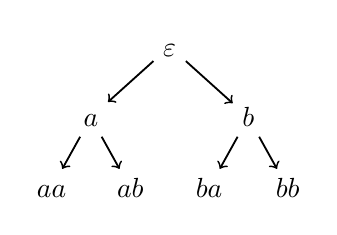
\begin{tikzpicture}
            \tikzset{
	level distance=.9cm,
	level 1/.style={sibling distance=2cm},
	level 2/.style={sibling distance=1cm},
	level 3/.style={sibling distance=.5cm},
	edge from parent/.style={draw, ->, line width=.66pt}
}

\node (t) {$\varepsilon\vphantom{b}$}
	child {node {$a\vphantom{b}$}
		child {node {$aa\vphantom{b}$}
		}
		child {node {$ab$}
		}
	}
	child {node {$b$}
		child {node {$ba$}
		}
		child {node {$bb$}
		}
	};
        \end{tikzpicture}
        \caption{\AP\label{fig:equal-length-plusone-relation}%
            The relation $\+R_2$ of \Cref{ex:equal-length-plusone},
            restricted to words of length at most 2.
        }
    \end{marginfigure}%
    \begin{marginfigure}%
        \centering
        \begin{tikzpicture}
            \tikzset{
	level distance=.9cm,
	level 1/.style={sibling distance=2.8cm},
	level 2/.style={sibling distance=1.4cm},
	level 3/.style={sibling distance=.7cm},
	edge from parent/.style={}
}

% Coloring
\fill[rounded corners, fill=cBlue, opacity=.5]
	(-2.5,-2.05) rectangle (2.5,-1.57)
	(-.3,-0.25) rectangle (.3,0.23);
\fill[rounded corners, fill=cYellow, opacity=.5]
	(-1.65,-1.15) rectangle (1.65,-0.67);
% Tree
\node (eps) {$\varepsilon\vphantom{b}$}
	child {node (a) {$a\vphantom{b}$}
		child {node (aa) {$aa\vphantom{b}$}
		}
		child {node (ab) {$ab$}
		}
	}
	child {node (b) {$b$}
		child {node (ba) {$ba$}
		}
		child {node (bb) {$bb$}
		}
	};
\draw[<->] (eps) edge (a)
	(eps) edge (b)
	(a) edge (aa)
	(a) edge (ab)
	(a) edge (ba)
	(a) edge (bb)
	(b) edge (aa)
	(b) edge (ab)
	(b) edge (ba)
	(b) edge (bb);
        \end{tikzpicture}
        \caption{\AP\label{fig:equal-length-plusone-incompatibility}%
            "Incompatibility graph" $\incompGraph{\+R_1}{\+R_2}$ and its "2-regular colouring".%
        }
    \end{marginfigure}%

    Note that while neither $\+R_1$ nor $\+R_2$ are "recognizable",
    they are "separable@@rel" by the "recognizable" relation
    $\+S$ consisting of all pairs $\tup{u,v}$ such that $|u|$ and $|v|$ have the same parity.
    Moreover, $\incompGraph{\+R_1}{\+R_2}$ is "2-regular colourable", the two colours being
    the words of even and odd length.
\end{example}

\begin{proposition}
    \AP\label{prop:incomp-is-automatic}
    If $\+R_1$ and $\+R_2$ are "automatic", then so is $\incompGraph{\+R_1}{\+R_2}$.
    Moreover, we can build an automaton for $\incompGraph{\+R_1}{\+R_2}$ in polynomial time in the size of the automata for $\+R_1$ and $\+R_2$.
\end{proposition}

\begin{proof}
    By definition, the "incompatibility relation" $\incompGraph{\+R_1}{\+R_2}$ can be written as
    $\+R_{\neg\compL} \cup \+R_{\neg\compLpr} \cup \+R_{\neg\compR} \cup \+R_{\neg\compRpr}$, where:
    \begin{align*}
        \+R_{\neg\compL} &\defeq \big\{ \tup{u,u'} \in \Sigma^* \times \Sigma^* \;\big\vert\; \exists v \in \Sigma^*,\; \tup{u,v} \in \+R_1 \land \tup{u',v} \in \+R_2 \big\} \text{,}\\
        \+R_{\neg\compLpr} &\defeq \big\{ \tup{u,u'} \in \Sigma^* \times \Sigma^* \;\big\vert\; \exists v \in \Sigma^*,\; \tup{u',v} \in \+R_1 \land \tup{u,v} \in \+R_2 \big\} \text{,}\\
        \+R_{\neg\compR} &\defeq \big\{ \tup{u,u'} \in \Sigma^* \times \Sigma^* \;\big\vert\; \exists v \in \Sigma^*,\; \tup{v,u} \in \+R_1 \land \tup{v,u'} \in \+R_2 \big\} \text{, and}\\
        \+R_{\neg\compRpr} &\defeq \big\{ \tup{u,u'} \in \Sigma^* \times \Sigma^* \;\big\vert\; \exists v \in \Sigma^*,\; \tup{v,u'} \in \+R_1 \land \tup{v,u} \in \+R_2 \big\}
    \end{align*}
    Observe that starting from automata for $\+R_1$ and $\+R_2$, then for each
    of the relation $\+R_{\neg\compL}$, $\+R_{\neg\compLpr}$, $\+R_{\neg\compR}$ or $\+R_{\neg\compRpr}$, we can build an "automaton@@sync" recognizing them
    using a product construction, which can be implemented in polynomial time.\footnote{More precisely, in this product construction the states are $Q_1 \times Q_2$
    where $Q_i$ is the set of states of an "automaton@@sync" $\+A_i$ for $\+R_i$. Then,
    for each transition
    \[
        q_i \transition{\tup{a,b}} q'_i
    \]
    in $\+A_i$
    ($i \in \{1,2\}$), we put a transition
    \[
        \tup{q_1,q_2} \transition{\tup{a,c}} \tup{q'_1,q'_2},
    \]
    with $a,b,c \in \Sigma\dcup\{\bot\}$. Potentially, this
    can produce transitions labelled by $\tup{\bot,\bot}$: we can get rid of those
    using the standard elimination of $\varepsilon$-transitions.
    Finally, a state $\tup{q_1,q_2}$ is accepting if $q_1$ and $q_2$ are accepting
    in $\+A_1$ and $\+A_2$, respectively.}
    It then follows that we can build a polynomial-size "automaton@@sync" recognizing
    $\incompGraph{R_1}{R_2}$ in polynomial time.
\end{proof}

We can now finish the proof of \Cref{thm:reg-colourability-equiv-separability}.

\begin{proof}[Proof of \eqref{item:reg-colourability-equiv-separability-1}.]
    \AP Given an instance $\tup{\+R_1,\+R_2}$ of the "$\REC$-separability problem", we
    reduce it to the "regular colourability problem" on its "incompatibility graph"
    $\incompGraph{\+R_1}{\+R_2}$.

    \proofcase{Left-to-right implication.} 
    Assume that there exists $\+S$ in $\kREC$ that "separates@@rel" $\+R_1$ from $\+R_2$.
    Then $\+S$ can be written as $(L_{i_1}\times L_{j_1}) \cup \cdots \cup (L_{i_\ell}\times L_{j_\ell})$, 
    where $(L_1,\hdots,L_k)$ is a partition of $\Sigma^*$ in $k$ "regular languages".
    We define the colour of a word $u \in \Sigma^*$ as the unique $i \in \lBrack 1,k \rBrack$
    "st" $u \in L_i$. In other words, the "colouring" is simply $\tup{L_1,\hdots,L_k}$. 

    This is indeed a proper "colouring": if $u$ and $u'$ have the same colour,
    we claim that $\tup{u,u'} \not\in \incompGraph{\+R_1}{\+R_2}$, "ie" that
    $u$ is "compatible" with $u'$. Indeed, take any $v \in \Sigma^*$: if $\tup{u,v} \in \+R_1$,
    then $\tup{u,v} \in \+S$, so $\tup{u,v} \in L_{i_m}\times L_{j_m}$ for some $m \in \lBrack 1,\ell\rBrack$. But since $u$ has the same colour 
    as $u'$, the fact that $u \in L_{i_m}$ implies $u' \in L_{i_m}$, and hence 
    $\tup{u',v} \in L_{i_m}\times L_{j_m}\subseteq \+S$.
    But $\+S$ "separates@@rel" $\+R_1$ from $\+R_2$, and therefore $\tup{u',v} \not\in \+R_2$.
    This tells us that \compL\ holds. The other conditions hold by symmetry.
    We conclude that $\tup{L_1,\hdots,L_k}$ defines
    a proper "$k$-colouring" of $\incompGraph{\+R_1}{\+R_2}$, that is "regular@regular colouring" since the $L_i$'s are "regular languages" by definition.

    \proofcase{Right-to-left implication.}
    Assume that $\incompGraph{\+R_1}{\+R_2}$ is "finitely regularly colourable", say by
    $\tup{L_1,\hdots,L_k}$. Then let $\+S$ be the union of all $\+S_i$'s ($i \in \lBrack 1,k\rBrack$) where
    \begin{align*}
        \+S_i \defeq\; & \{\tup{u,v} \mid u \in L_i \text{ and } \tup{u',v} \in \+R_1 \text{ for some } u' \in L_i \}\\
        & \cup \{\tup{u,v} \mid v \in L_i \text{ and } \tup{u,v'} \in \+R_1 \text{ for some } v' \in L_i \}.  
    \end{align*}
    Since $\bigcup_i L_i = \Sigma^*$, we get $\+R_1 \subseteq \+S$.
    Moreover, we claim that $\+R_2 \cap \+S = \emptyset$. Indeed, if $\tup{u,v} \in \+S$,
    then $\tup{u,v} \in \+S_i$ for some $i \in \lBrack 1,k\rBrack$. It either means that
    (1) $u\in L_i$ and $\tup{u',v} \in \+R_1$ for some $u' \in L_i$, or
    (2) $v\in L_i$ and $\tup{u,v'} \in \+R_2$
    for some $v' \in L_i$. In case (1), $u$ and $u'$
    have the same colour, and since $\tup{L_1,\hdots,L_k}$ is a "colouring"
    of $\incompGraph{\+R_1}{\+R_2}$, $u$ must be "compatible" with $u'$.
    The assumption $\tup{u',v} \in \+R_1$ together with \compLpr\ then yields
    that $\tup{u,v} \not\in \+R_2$. The other case is symmetric.
    Therefore, $\tup{u,v} \not\in \+R_2$, and thus $\+S$ "separates@@rel" $\+R_1$ from $\+R_2$.

    Finally, we show that $\+S$ is "recognizable". In fact, 
    \[
        \+S = \bigcup_{i=1}^k \bigl(
            L_i \times \+R_1[L_i]
        \bigr) \cup \bigl(
            \+R_1^{-1}[L_i] \times L_i
        \bigr),
    \] 
    where for any set $X \subseteq \Sigma^*$ we define $\+R_1[X]$ (resp. $\+R_1^{-1}[X]$)
    to be the set of $v\in \Sigma^*$ (resp. $u \in \Sigma^*$) such that
    $\tup{u,v} \in \+R_1$ for some $u \in X$ (resp. $v\in X$).
    Hence, $\+R_1$ and $\+R_2$ are $\REC$-"separable@@rel".%
    \footnote{%
        Note however that $\+S$ does not necessarily belong to $\kREC$,
        but \emph{a priori} to $\kREC[8^k]$: indeed, from the
        $L_i$'s, $\+R_1[L_i]$'s and $\+R_1^{-1}[L_i]$'s,
        one can produce using a powerset construction a partition of $\Sigma^*$
        in $2^{3k} = 8^k$ "regular languages" "st" any $L_i$ (resp. $\+R_1[L_i]$,
        resp. $\+R_1^{-1}[L_i]$) can be written as the union of some of these languages.
    }
\end{proof}

Motivated by these reductions, we focus our attention to "regular colourings" of "rational graphs",
eventually proving that both the "$k$-regular colourability@@problem" and
"regular colourability problems@regular colourability problem" are undecidable.

\subsection{$k$-Regular Colourability Problem}

While we do not know how to approach the "regular colourability problem", we show that as soon as we add the restriction that the number of colours is bounded, the problem becomes undecidable;
"ie", the "$k$-regular colourability problem" is undecidable for $k\geq 2$. Using this, we obtain in the next section 
the undecidability for the separability problem on two natural classes of 
"recognizable relations". This is proven by a reduction from a suitable problem on reversible 
Turing Machines with certain restrictions, which we call ``well-founded''.

\paragraph*{Regularity of Reachability for Turing Machines.}
We use the standard notation $u[i..j]$ to denote the factor of a word $u$ between (and including) positions $i$ and $j$, and $u[i]$ to denote $u[i..i]$.
%\sidediego{Should this go the preliminaries?}
Consider any deterministic Turing Machine (TM) $T = \tup{Q,\Gamma,\bot,\delta,q_0,F}$, where $Q$ is the set of states, $\Gamma$ is tape alphabet, $\bot$ is the blank symbol, $\delta: (Q \setminus F) \times \Gamma_\bot \to Q \times \Gamma \times \set{L,R}$ is the transition (partial) function, where $\Gamma_\bot = \Gamma \cup \set\bot$, and $q_0$ and $F$ is the initial and set of final states, respectively.
%
We represent a configuration with tape content $w \cdot \bot^\omega$ (where $w \in \Gamma^* \cdot \set{\bot}$), in state $q$ and with the head pointing to the cell number $1 \leq i \leq |w|$, as the string
\[
   w[1..i-1] \cdot (w[i],q) \cdot w[i+1..|w|] 
\]
over the alphabet $\Sigma_T = \Gamma \cup (\Gamma_\bot \times Q)$.
\AP In light of this representation, we will henceforth denote by ``configuration'' any string from the set  $\intro*\configs \defeq (\Gamma^* \cdot (\Gamma_\bot \times Q)) \cup  (\Gamma^* \cdot (\Gamma \times Q) \cdot \Gamma^*)$. The ""initial configuration"" is $(\bot,q_0)$.
\AP The ""configuration graph"" of $T$ is the infinite graph $\intro*\confGraph$ having $\configs$ as set of vertices and an edge from $c$ to $c'$, denoted $c \rightarrow c'$, if $c'$ is the configuration of the next step of $T$ starting from $c$. Observe that the "configuration graph" $\confGraph$ of any TM $T$ is an effective "synchronous graph" (see, e.g., \cite{KuskeLohrey2010AutomaticGraphs}).

\AP We say that a deterministic TM $T$ is ""reversible"" if every node of $\confGraph$ has in-degree at most 1, in other words if the machine is co-deterministic\footnote{Note
that a modern proof of undecidability of the isomorphism problem for automatic structures by
Blumensath \cite[\S VIII. Theorem 4.3, p. 396 \& second claim, p. 398]{Blumensath2023MSO} also relies on the use of "reversible" Turing machines.}.
We say that a TM $T$ is a ""well-founded Reversible Turing Machine"" (\reintro{wf-RTM}) if its "configuration graph" is such that (1) the "initial configuration" has in-degree 0 (2) every node has in-degree and out-degree at most one (3) there are no infinite backward paths $c_1 \leftarrow c_2 \leftarrow \dotsb$ in $\confGraph$. 

\AP Note that every "well-founded Reversible Turing Machine" is deterministic and "reversible" and, moreover,
its "configuration graph" is a (possibly infinite) disjoint union of
directed paths, which are all finite, or isomorphic to $(\mathbb{N}, +1)$.
The set of ""reachable configurations"", denoted by $\intro*\Reach$, is 
the set of all configurations that admit a path from the "initial configuration"
% the set of all "configurations" in the connected component of the "initial configuration" 
in $\confGraph$, for a given TM $T$.
Such a configuration graph is depicted on \Cref{subfig:config-graph-wf-RTM}.

\AP The ""reachable regularity problem"" is the problem of, given a "wf-RTM" $T$, whether its set of "reachable configurations" is a regular language. To show that is it undecidable, we exhibit a reduction from the halting problem on deterministic "reversible" Turing machines.

\begin{proposition}[{\cite[Theorem 1]{Lecerf1963MachinesReversibles}}]
    \AP\label{prop:halting-problem-detrevTM}
    The halting problem on deterministic "reversible" Turing machines is undecidable.
\end{proposition}

For more details and pointers on "reversible" Turing machines, see \cite[Chapter 5]{Morita2017Reversible}.

\begin{lemma}
    \AP\label{lem:reachable-regularity}
    The "reachable regularity problem" is undecidable.
\end{lemma}

\begin{proof}[Proof sketch]
    By reducing the halting problem on deterministic "reversible" Turing machines,
    in such a way that the "reachable configurations" whose
    state $q$ coincide with the state of the original machine are
    of the form $(u q v a^n b^n)$ where $(u q v)$ is a configuration of the original machine,
    $a$ and $b$ are new symbols,
    and $n\in\N$. Transitions are defined in such a way that the new machine is a
    "wf-RTM": this is implemented by having, for every transition $uqv \to u'q'v'$ of the original machine and every $n\in \N$, a (multi-step) transition $(u q v a^n b^n) \to^* (u' q' v' a^{n+1} b^{n+1})$---and is illustrated in \Cref{fig:reachable-regularity}.
	\begin{figure}[htb]
		\centering
        \begin{tikzpicture}
		    % ---
% First tape
% ---
\node (0) at (0,0) {0};
\node[right = 0cm of 0] (1) {0};
\node[right = 0cm of 1] (2) {1};
\node[right = 0cm of 2] (3) {0};
\node[right = 0cm of 3] (4) {1};
\node[right = 0cm of 4] (5) {$\triangleright$};
\node[right = 0cm of 5] (6) {$\triangleright$};
\node[right = 0cm of 6] (7) {$\triangleright$};
\node[right = 0cm of 7] (8) {$\triangleleft$};
\node[right = 0cm of 8] (9) {$\triangleleft$};
\node[right = 0cm of 9] (10) {$\triangleleft$};

\draw[rounded corners=4pt] (0.south west) rectangle (10.north east);
\draw[->, thick] ($(5.north)+(0,.4)$) -- ($(5.north)+(0,.1)$);
\node[above=.05cm, circle, draw=cBlue, fill=cBlue, opacity=.5, text opacity=1, inner sep=1.5pt] at ($(5.north)+(0,.4)$) {$p$};

% ---
% Second tape
% ---
\node[below = 1.2cm of 0] (0') {0};
\node[right = 0cm of 0'] (1') {0};
\node[right = 0cm of 1'] (2') {1};
\node[right = 0cm of 2'] (3') {0};
\node[right = 0cm of 3'] (4') {1};
\node[right = 0cm of 4'] (5') {1};
\node[right = 0cm of 5'] (6') {$\triangleright$};
\node[right = 0cm of 6'] (7') {$\triangleright$};
\node[right = 0cm of 7'] (8') {$\triangleleft$};
\node[right = 0cm of 8'] (9') {$\triangleleft$};
\node[right = 0cm of 9'] (10') {$\triangleleft$};

\draw[rounded corners=4pt] (0'.south west) rectangle (10'.north east);
\draw[->, thick] ($(6'.north)+(0,.4)$) -- ($(6'.north)+(0,.1)$);
\node[above=.05cm, circle, draw=cRed, fill=cRed, opacity=.5, text opacity=1, inner sep=1.5pt] at ($(6'.north)+(0,.4)$) {$\phantom{q}$};

% ---
% Third tape
% ---
\node[below = 1.2cm of 0'] (0'') {0};
\node[right = 0cm of 0''] (1'') {0};
\node[right = 0cm of 1''] (2'') {1};
\node[right = 0cm of 2''] (3'') {0};
\node[right = 0cm of 3''] (4'') {1};
\node[right = 0cm of 4''] (5'') {1};
\node[right = 0cm of 5''] (6'') {$\triangleright$};
\node[right = 0cm of 6''] (7'') {$\triangleright$};
\node[right = 0cm of 7''] (8'') {$\triangleright$};
\node[right = 0cm of 8''] (9'') {$\triangleright$};
\node[right = 0cm of 9''] (10'') {$\triangleleft$};

\draw[rounded corners=4pt] (0''.south west) rectangle (10''.north east);
\draw[->, thick] ($(10''.north)+(0,.4)$) -- ($(10''.north)+(0,.1)$);
\node[above=.05cm, circle, draw=cRed, fill=cRed, opacity=.5, text opacity=1, inner sep=1.5pt] at ($(10''.north)+(0,.4)$) {$\phantom{q}$};

% ---
% Fourth tape
% ---
\node[below = 1.2cm of 0''] (0''') {0};
\node[right = 0cm of 0'''] (1''') {0};
\node[right = 0cm of 1'''] (2''') {1};
\node[right = 0cm of 2'''] (3''') {0};
\node[right = 0cm of 3'''] (4''') {1};
\node[right = 0cm of 4'''] (5''') {1};
\node[right = 0cm of 5'''] (6''') {$\triangleright$};
\node[right = 0cm of 6'''] (7''') {$\triangleright$};
\node[right = 0cm of 7'''] (8''') {$\triangleright$};
\node[right = 0cm of 8'''] (9''') {$\triangleright$};
\node[right = 0cm of 9'''] (10''') {$\triangleleft$};
\node[right = 0cm of 10'''] (11''') {$\triangleleft$};
\node[right = 0cm of 11'''] (12''') {$\triangleleft$};
\node[right = 0cm of 12'''] (13''') {$\triangleleft$};

\draw[rounded corners=4pt] (0'''.south west) rectangle (13'''.north east);
\draw[->, thick] ($(13'''.north)+(0,.4)$) -- ($(13'''.north)+(0,.1)$);
\node[above=.05cm, circle, draw=cRed, fill=cRed, opacity=.5, text opacity=1, inner sep=1.5pt] at ($(13'''.north)+(0,.4)$) {$\phantom{q}$};

% ---
% Fifth tape
% ---
\node[below = 1.2cm of 0'''] (0'''') {0};
\node[right = 0cm of 0''''] (1'''') {0};
\node[right = 0cm of 1''''] (2'''') {1};
\node[right = 0cm of 2''''] (3'''') {0};
\node[right = 0cm of 3''''] (4'''') {1};
\node[right = 0cm of 4''''] (5'''') {1};
\node[right = 0cm of 5''''] (6'''') {$\triangleright$};
\node[right = 0cm of 6''''] (7'''') {$\triangleright$};
\node[right = 0cm of 7''''] (8'''') {$\triangleright$};
\node[right = 0cm of 8''''] (9'''') {$\triangleright$};
\node[right = 0cm of 9''''] (10'''') {$\triangleleft$};
\node[right = 0cm of 10''''] (11'''') {$\triangleleft$};
\node[right = 0cm of 11''''] (12'''') {$\triangleleft$};
\node[right = 0cm of 12''''] (13'''') {$\triangleleft$};

\draw[rounded corners=4pt] (0''''.south west) rectangle (13''''.north east);
\draw[->, thick] ($(6''''.north)+(0,.4)$) -- ($(6''''.north)+(0,.1)$);
\node[above=.05cm, circle, draw=cBlue, fill=cBlue, opacity=.5, text opacity=1, inner sep=1.5pt] at ($(6''''.north)+(0,.4)$) {$q$};

% ---
% Transitions
% ---
\draw[->, dashed] ($(10.east)+(.3,-.2)$) to[bend left=50]
	node[midway, right=.15cm, align=left, text width=3.5cm, font=\footnotesize] {simulate $T$}
	($(10'.east)+(.3,.2)$);

\draw[->, dashed] ($(10'.east)+(.3,-.2)$) to[bend left=50]
	node[midway, right=.15cm, align=left, text width=3.5cm, font=\footnotesize]
		{overwrite the first two $\triangleleft$'s with $a$'s}
	($(10''.east)+(.3,.2)$);

% \draw[-, dashed] ($(10''.east)+(.3,-.1)$) to ($(10''.east)+(1.5,-.1)$);
\draw[->, dashed] ($(10''.east)+(1.5,-.2)$) to[bend left=50]
	node[midway, right=.15cm, align=left, text width=3.5cm, font=\footnotesize]
		{append three $\triangleleft$'s}
	($(13'''.east)+(.3,.2)$);


\draw[->, dashed] ($(13'''.east)+(.3,-.2)$) to[bend left=50]
	node[midway, right=.15cm, align=left, text width=3.5cm, font=\footnotesize]
		{go back to the new position, in the new state}
	($(13''''.east)+(.3,.2)$);
        \end{tikzpicture}
		\caption{
			\AP\label{fig:reachable-regularity}
			Encoding of a single transition of the form
			``when reading a blank in state $\color{cBlue} p$, write a
			$1$, go in state $\color{cBlue} q$ and move right''
			of the machine $T$ in the machine $T'$
			in the proof of \Cref{lem:reachable-regularity}.
			Red unlabelled states represent states of $T'$
			that are not originally present in $T$.
		}
	\end{figure}
	Moreover:
    \begin{itemize}
        \item if the original machine was halting, then the "reachable configurations"
            of the new one are finite and hence regular;
        \item otherwise, the set of "reachable configurations" is not regular,
            which follows from the non-regularity of any infinite subset of $\{a^n b^n \mid n \in \N\}$.
    \end{itemize}
\end{proof}

\begin{proof}
    By reduction from the halting problem for deterministic and "reversible" TMs, which is undecidable by \Cref{prop:halting-problem-detrevTM}. Given a deterministic and "reversible" TM $T$ (running on the empty input), consider the TM $T'$ where every time there is a transition $(u, p, v) \to (u', q, v')$ from configuration $c$ to configuration $c'$ in $T$,
	simulate this transition in $T'$---$a$'s should be treated as blank symbols---,
	and then rewrite $a^n b^n$ into $a^{n+1}b^{n+1}$.
	When $T$ writes on a blank symbol that was actually a $a$ in $T'$,
	we must also add an extra $a$ (to account for the one that was overwritten):
	this case is depicted \Cref{fig:reachable-regularity}.
	Moreover, when $T$ deletes a symbol at the end of the tape,
	we must shift the $a^n b^n$ prefix. This can be done by replacing the blank
	with an $a$, the last $a$ with a $b$, and deleting the last $b$.
	
	% in \Cref{fig:reachable-regularity}, by a series of steps that ``make some room'' between $c$ and $c'$ if needed (for example because the head was at the last position of $c$ and moves to the right), and make some room between the $a$'s and the $b$'s to accomodate for the extra $a$, and writes an extra $b$ at the end. This can be done with the invariant that at all times there are roughly as many $a$'s as $b$'s ($\pm 1$) in the working tape.
    Observe that $T'$ is a "wf-RTM":
    \begin{enumerate}
        \item the "initial configuration" $(\bot,q_0,\bot)$ has no predecessor;
        \item it is deterministic and co-deterministic:
        \begin{itemize}
            \item every configuration inside a path $(u, q, v a^n b^n) \xrightarrow{*} (u, q, v a^{n+1} b^{n+1})$ 
            has, by definition, exactly in- and out-degree one;
            \item every configuration of the form $(u, p, v a^n b^n)$ has as many predecessors 
            [resp. successors] in $T'$ as $(u,q,v)$ in $T$, namely one since $T$ was assumed to be
                deterministic and "reversible";
        \end{itemize}
        \item it has no infinite descending chain since $\N$ is well-founded.
    \end{enumerate}
    Moreover, $T'$ has no cycle,
    so if $T$ is halting (on an empty input) then the set of "reachable configurations" of $T'$ is finite (since it is a "wf-RTM") and thus regular. If $T$ is not halting, the set of "reachable configurations" of $T'$ is infinite and its projection onto $\set{a,b}$ is an infinite set of words of the form $a^{n} b^{n'}$ where $n-2 \leq n' \leq n+2$. Hence, since regular languages are closed under homomorphic images, the "reachable configurations" of $T'$ cannot be regular.
\end{proof}


\paragraph*{Undecidability of the $k$-Regular Colourability Problem.}
We can now show undecidability for the "$k$-regular colourability problem" by reduction from the "reachable regularity problem" as defined before.

\begin{fact}
    \AP\label{fact:initial-nodes-are-regular}
    Given an "synchronous graph", the set of nodes with no predecessor is effectively a regular language. 
\end{fact}

\begin{theorem}
    \AP\label{thm:k-reg-col-undec}
    The "$k$-regular colourability problem" on "synchronous graphs" is undecidable, for every $k\geq 2$. More precisely, the problem is recursively enumerable-complete. This holds also for connected "synchronous graphs".
\end{theorem}

\begin{proof}%
    \begin{marginfigure}%
        \centering
        \begin{tikzpicture}
            % Reachable configuration
\fill[rounded corners, draw=cGreen, fill=cGreen, opacity=.3]
	(-.3,-.3) rectangle (2.75, .3);
% Initial configuration
\fill[rounded corners, draw=cYellow, fill=cYellow, opacity=.3]
	(-.3,.3) rectangle (.3, -1.95);

% First line
\node[vertex] (a0) at (0,0) {};
\foreach \i in {0,...,2} {
	\pgfmathtruncatemacro{\next}{\i + 1}
	\node[vertex, right = of a\i] (a\next) {};
	\draw[edge] (a\i) to (a\next);
}

% Second line
\node[vertex, below = of a0] (b0) {};
\foreach \i in {0,...,3} {
	\pgfmathtruncatemacro{\next}{\i + 1}
	\node[vertex, right = of b\i] (b\next) {};
	\draw[edge] (b\i) to (b\next);
}
\node[draw=none, fill=none, right = 0cm of b4] (binf) {$\cdots$};

% Third line
\node[vertex, below = of b0] (c0) {};
\foreach \i in {0,1} {
	\pgfmathtruncatemacro{\next}{\i + 1}
	\node[vertex, right = of c\i] (c\next) {};
	\draw[edge] (c\i) to (c\next);
}

% Labels
\node[draw=none, fill=none, font=\small] [below = 1em of c0] {$\GermC{cYellow}$};
\node[draw=none, fill=none, font=\small, align=center] [above = 1em of $(a1)!0.5!(a2)$]
	{$\ReachC{\+T}{cGreen}$};
        \end{tikzpicture}
        \caption{
            \AP\label{fig:reduction-wf-RTM-to-colouring-config-graph-wf-RTM}
            Configuration graph of a "well-founded Reversible Turing Machine".
        }
    \end{marginfigure}%
    \begin{marginfigure}
        \centering
        \begin{tikzpicture}
            
% Reachable configuration
\fill[rounded corners, draw=cGreen, fill=cGreen, opacity=.3]
	(-.3,-.9) rectangle (2.75, .3);
% Initial configuration
\fill[rounded corners, draw=cYellow, fill=cYellow, opacity=.3]
	(-.3,.3) rectangle (.3, -3.8);

% First line
\node[vertex, cBlue, fill=cBlue, fill opacity=.4] (a0) at (0,0) {};
\node[vertex, cRed, fill=cRed, fill opacity=.4] (a'0) [below = .3cm of a0] {};
\draw[edge, densely dotted] (a0) to (a'0);
\foreach \i in {0,...,2} {
	\pgfmathtruncatemacro{\next}{\i + 1}
	\node[vertex, cBlue, fill=cBlue, fill opacity=.4, right = of a\i] (a\next) {};
	\node[vertex, cRed, fill=cRed, fill opacity=.4, right = of a'\i] (a'\next) {};
	\draw[edge] (a'\i) to (a\next);
	\draw[edge, densely dotted] (a\next) to (a'\next);
}

% Second line
\node[vertex, cBlue, fill=cBlue, fill opacity=.4, below = of a'0] (b0) {};
\node[vertex, cRed, fill=cRed, fill opacity=.4, below =.3cm of b0] (b'0) {};
\draw[edge, densely dotted] (b0) to (b'0);
\foreach \i in {0,...,3} {
	\pgfmathtruncatemacro{\next}{\i + 1}
	\node[vertex, cBlue, fill=cBlue, fill opacity=.4, right = of b\i] (b\next) {};
	\node[vertex, cRed, fill=cRed, fill opacity=.4, right = of b'\i] (b'\next) {};
	\draw[edge] (b'\i) to (b\next);
	\draw[edge, densely dotted] (b\next) to (b'\next);
}
\node[draw=none, fill=none, right = .6em of $(b4)!0.5!(b'4)$] (binf) {$\cdots$};

% Third line
\node[vertex, cBlue, fill=cBlue, fill opacity=.4, below = of b'0] (c0) {};
\node[vertex, cRed, fill=cRed, fill opacity=.4, below = .3cm of c0] (c'0) {};
\draw[edge, densely dotted] (c0) to (c'0);
\foreach \i in {0,1} {
	\pgfmathtruncatemacro{\next}{\i + 1}
	\node[vertex, cBlue, fill=cBlue, fill opacity=.4, right = of c\i] (c\next) {};
	\node[vertex, cRed, fill=cRed, fill opacity=.4, right = of c'\i] (c'\next) {};
	\draw[edge] (c'\i) to (c\next);
	\draw[edge, densely dotted] (c\next) to (c'\next);
}

% Edges between Init nodes
\draw[edge, densely dashed] (a0) to[bend right] (b0);
\draw[edge, densely dashed] (a0) to[bend right] (c0);

% Labels
\node[draw=none, fill=none, cYellow, font=\footnotesize, align=left]
	[below right = 1em and -1em of $(c'0)$]
	{nodes originating from	$\GermC{\+T}{cYellow}$};
\node[draw=none, fill=none, cGreen, font=\footnotesize, align=left]
	[above right = 1em and -1em of $(a0)$]
	{nodes originating from $\ReachC{\+T}{cGreen}$};
        \end{tikzpicture}
        \caption{
            \AP\label{subfig:reduction-wf-RTM-to-colouring}
            The synchronous graph to which the "configuration graph"
            of \Cref{fig:reduction-wf-RTM-to-colouring-config-graph-wf-RTM} is reduced.
        }
    \end{marginfigure}%
	\proofcase{Lower bound.}
    By reduction from the "reachable regularity problem" for "wf-RTM"s
    (\Cref{lem:reachable-regularity}). We first show it for $k=2$.
    \AP Given a "wf-RTM" $T$, let $c_{\textit{init}}$ be its "initial configuration".
    Observe that the set $\intro*\Init$ of all vertices of $\confGraph$ with in-degree $0$ is an effective regular language (by \Cref{fact:initial-nodes-are-regular}), and that $c_{\textit{init}} \in \Init$. Let $B$ and $R$ be fresh symbols. 
    Consider the "synchronous graph" $\AutGraph{L}{E}$ for $L = \set{B,R} \times \configs$, having 
    an edge from $(z,c) \in \{B,R\} \times \configs$ to $(z',c') \in \{B,R\} \times \configs$ if either 
    \begin{enumerate}
        \item $(z,z') = (B,R)$ and $c=c'$;
        \item $(z,z') = (R,B)$ and there is an edge from $c$ to $c'$ in $\confGraph$; or
        \item $(z,z') = (B,B)$, $c = c_{\textit{init}}$ and $c' \in \Init \setminus \set{c_{\textit{init}}}$.
    \end{enumerate}
Fresh symbols $B$ and $R$ are utilized to represent two versions of each configuration - one in Blue and one in Red. This graph is depicted
    on \Cref{fig:reduction-wf-RTM-to-colouring}.
    Note that $\AutGraph{L}{E}$ is connected and "2-colourable": in fact, it is a directed (possibly infinite) tree with root $(B,c_{\textit{init}})$. 
    
    We claim that $\AutGraph{L}{E}$ is "$2$-regular colourable" if, and only if, the set of "reachable configurations" of $T$ is a regular language. 
    In fact, up to permuting the two-colours, 
  $\AutGraph{L}{E}$ admits a unique 2-colouring, defined by:
    \[
        C_1 ~~ \defeq ~~ \{B\} \times \Reach ~~\cup~~ \{R\} \times (\configs \setminus \Reach)
    \]
    and $C_2$ is the complement of $C_1$.
    If $\Reach$ is regular, then so is $C_1$. Dually, if $C_1$ is regular, then
    $\Reach$ is the set of configurations $c$ such that $(B,c) \in C_1$ and hence is regular.
    It follows that $\AutGraph{\Sigma^*}{E}$ is "$2$-regular colourable" if and only if
    the "reachable configurations" of $T$ are regular, which concludes the proof for $k=2$.

    % In one direction, if the "reachable configurations" of $T$ is a regular language $L$, then consider the regular sets of vertices of $G$ defined as $C_1 = (\set B \times L) \cup (\set R \times (\configs \setminus L))$ and $C_2$ as its complement. It is easy to verify that $(C_1,C_2)$ is a "two-regular colouring@$k$-regular colouring" of $\AutGraph[E]$.

    % In the converse direction, suppose there is a "two-regular colouring@$k$-regular colouring" $(C_1,C_2)$ of $\AutGraph[E]$, and suppose without loss of generality that $(B,c_{\textit{init}}) \in C_1$. Since $\AutGraph[E]$ is connected, the colouring is uniquely determined by the colour of any of its vertices, and hence $C_1 = (\set B \times \hat L) \cup (\set R \times (\configs \setminus \hat L))$, where $\hat L$ is the set of "reachable configurations" of $T$. Now $\hat L$ can be obtained from $C_1$ by means of projection and thus $\hat L$ is regular.

    To prove the statement for any $k>2$, we define $\AutGraph{L}{E_k}$ as the result of adding a $(k-2)$-clique to $\AutGraph{L}{E}$ and adding an edge from every vertex of the clique to every vertex incident to an edge of $E$. This forces the clique to use $k-2$ colours that cannot be used in the remaining part of the graph and the proof is then analogous.

	\proofcase{Upper-bound.} We show that the problem is recursively enumerable. Let us define a $k$-coloured automaton like a regular (complete) DFA, except that instead of having
	a set of final states, it has a partition $\langle C_1,\hdots,C_k \rangle$ of its states.
	Such an automaton recognizes a regular colouring $\Sigma^* \to \set{1, \dotsc, k}$.
	Given an "synchronous graph" $\AutGraph{L}{R}$---specified by
	 NFA's $\+A_1$ and $\+A_2$ recognizing $L$ and $\convolRel{R}$  respectively--- and a $k$-coloured automaton $\+B$,
	we can build, by a product construction, an NFA $\+A'_2$  which accepts
	all $u \otimes v \in \convolRel{R}$ such that the colour of $u$ is distinct from the colour of $v$.
	Then, $\+A'_2$ is equivalent to $\+A_2$ if, and only if, $\+B$ describes a proper "$k$-colouring" 
	of $\AutGraph{L}{R}$. The "RE" upper-bound of the "$k$-regular colourability problem" follows: it 
	suffices to enumerate all $k$-coloured automata and check for equivalence.
\end{proof}

Note that this reduction provides an easy way of building
graphs in the shape of \Cref{subfig:reduction-wf-RTM} that are "2-colourable" (in fact, they are trees) but not "2-regular colourable". In fact, we can provide a slightly more
direct construction.

\begin{example}
    \AP\label{ex:tree-not-2-reg-colourable}
    On the alphabet $\Sigma = \{a,b\}$, the tree $\+T$ depicted in \Cref{fig:tree-not-2reg-colour} whose set of vertices is $V = a^*b^*$ and whose set 
    of edges is $E = E_{\mathrm{incr}} \cup E_{\mathrm{init}}$, with 
    \begin{align*}
        E_{\mathrm{incr}} & = \{(a^pb^q,\, a^{p+1}b^{q+1}) \mid p,q \in \N\} \\
        E_{\mathrm{init}} & = \{(\varepsilon,\, a^p) \mid p \in \N\} \cup \{(\varepsilon,\, b^q) \mid q \in \N\}, 
    \end{align*}    
    is "automatic" but not "2-regular colourable". 
    Indeed, its only "2-colouring"
    consists in partitioning the vertices of $\+T$ into
    \[
        C = \{a^n b^n \mid n \in 2\N\}
            \cup \{a^p b^q \mid p > q \text{ and $q$ is odd}\}
            \cup \{a^p b^q \mid p < q \text{ and $p$ is odd}\}
    \]
    and its complement $V \setminus C$.
    Let $P = \{a^p b^q \mid p, q \in 2\N\} = (aa)^*(bb)^*$:
    $P$ is regular, yet $C \cap P = \{a^n b^n \mid n \in 2\N\}$ is not.
    Hence, $C$ is not regular, and thus $\+T$ is not "2-regular colourable".
    \qed 
\end{example}

\begin{figure}[htb]
    \centering
    \begin{tikzpicture}
        % Coloring
\fill[rounded corners, fill=cBlue, opacity=.5]
	(-.4,-0.25) rectangle (.4,0.23)
	(2.1,-0.25) rectangle (2.9,0.23)
	(0.85,-0.52) rectangle (1.65, -2.5)
	(3.35,-0.52) rectangle (4.15, -2.5);

\fill[rounded corners, fill=cRed, opacity=.5, xshift=1.25cm]
	(-.4,-0.25) rectangle (.4,0.23)
	(2.1,-0.25) rectangle (2.9,0.23);
\fill[rounded corners, fill=cRed, opacity=.5, xshift=-1.25cm]
	(0.85,-0.52) rectangle (1.65, -2.5)
	(3.35,-0.52) rectangle (4.15, -2.5);

% Tree
\node (eps) at (0,0) {$\varepsilon$};
\node (ab) at (1.25,0) {$ab$};
\node (aabb) at (2.5,0) {$a^2b^2$};
\node (aaabbb) at (3.75,0) {$a^3b^3$};

\node (a) at (0,-.75) {$a$};
\node (aab) at (1.25,-.75) {$aab$};
\node (aaabb) at (2.5,-.75) {$a^3b^2$};
\node (aaaabbb) at (3.75,-.75) {$a^4b^3$};

\node (b) at (0,-1.5) {$b$};
\node (abb) at (1.25,-1.5) {$abb$};
\node (aabbb) at (2.5,-1.5) {$a^2b^3$};
\node (aaabbbb) at (3.75,-1.5) {$a^3b^4$};

\node (aa) at (0,-2.25) {$aa$};
\node (aaab) at (1.25,-2.25) {$a^3b$};
\node (aaaabb) at (2.5,-2.25) {$a^4b^2$};
\node (aaaaabbb) at (3.75,-2.25) {$a^5b^3$};

\draw[->] (eps) to (ab);
\draw[->] (ab) to (aabb);
\draw[->] (aabb) to (aaabbb);
\draw[->, dashed] (aaabbb) to ($(aaabbb)+(1,0)$);

\draw[->] (a) to (aab);
\draw[->] (aab) to (aaabb);
\draw[->] (aaabb) to (aaaabbb);
\draw[->, dashed] (aaaabbb) to ($(aaaabbb)+(1,0)$);

\draw[->] (b) to (abb);
\draw[->] (abb) to (aabbb);
\draw[->] (aabbb) to (aaabbbb);
\draw[->, dashed] (aaabbbb) to ($(aaabbbb)+(1,0)$);

\draw[->] (aa) to (aaab);
\draw[->] (aaab) to (aaaabb);
\draw[->] (aaaabb) to (aaaaabbb);
\draw[->, dashed] (aaaaabbb) to ($(aaaaabbb)+(1,0)$);

\draw[->] (eps) edge[bend right=40] (a)
	edge[bend right=40] (b)
	edge[bend right=40] (aa)
	edge[dashed, bend right=40] ($(aa)+(0,-.75)$);

\node[below = .25cm of aaab, color=cBlue] {$C$}; 
\node[below = .25cm of aaaabb, color=cRed] {$V \setminus C$}; 
    \end{tikzpicture}
    \caption{
        \label{fig:tree-not-2reg-colour}
        The "automatic tree@synchronous graph" $\+T$ of \Cref{ex:tree-not-2-reg-colourable},
        and its unique "2-colouring" $(C, V\setminus C)$, which is not "regular@@colouring".
    }
\end{figure}
\subsection{Bounded Recognizable Relations}
\AP\label{sec:dichotomy-bounded}

\paragraph*{Separability for Bounded Recognizable Relations.}

In this part, we capitalize on the undecidability result of \Cref{sec:dichotomy-k-regular-colourability}, showing how this implies the undecidability for the separability problem on two natural classes of bounded "recognizable relations", namely $\kREC$ and $\kPROD$.
For any $k$, $\reintro*\kPROD$ is the subclass of $\REC$ consisting of unions of $k$ Cartesian products of "regular languages" (which is a subclass of $\kREC[2^{2k}]$).

First, observe that the "$\kREC[1]$-separability problem" is trivially decidable, since the only possible "separator@@rel" is $\Sigma^* \times \Sigma^*$. However, for any other $k>1$, the problem is undecidable.

\begin{corollary}
    \label{coro:krec-sep-undec}
    The "$\kREC$-separability problem" is undecidable, for every $k>1$.
\end{corollary}

\begin{proof}
    This is a consequence of the reduction from the "$k$-regular colourability problem" of \Cref{thm:reg-colourability-equiv-separability}, combined with the undecidability of the latter for every $k>1$ (\Cref{thm:k-reg-col-undec}).
\end{proof}

On the $\kPROD$ hierarchy we will find the same phenomenon. In particular the case $k=1$ is also trivially decidable.

\begin{proposition}
    The "$\kPROD[1]$-separability problem" is decidable.
\end{proposition}
\begin{proof}
    Given two "automatic relations" $\+R_1, \+R_2$, there exists $S \in $ \kPROD[1]
    that "separates@@rel" $\+R_1$ from $\+R_2$ if and only if $\pi_1(\+R_1)\times \pi_2(\+R_1)$
    "separates@@rel" $\+R_1$ from $\+R_2$.\footnote{Here,
    \(
        \pi_1(\+R_1) \defeq 
        \{u \in \Sigma^* \mid \exists v\in \Sigma^*,\,\tup{u,v} \in \+R_1\},
    \)
    and similarly,
    \(
        \pi_2(\+R_1) \defeq 
        \{v \in \Sigma^* \mid \exists u\in \Sigma^*,\,\tup{u,v} \in \+R_1\}.
    \)
    Both languages can be effectively computed from $\+R_1$.}
\end{proof}

As soon as $k>1$, the "$\kPROD$-separability problem" becomes undecidable.

\begin{lemma}
    A "symmetric@@rel" "automatic relation" $\+R$ and the identity $\Id$ are "separable@@rel" by a relation in $\kPROD[2]$ iff they have a "separator@@rel" of the form $(A \times B) \cup (B \times A)$.
\end{lemma}
\begin{proof}
    Assume that $\+S \in \kPROD[2]$ "separates@@rel" $\+R$ from $\Id$.
    Then $\+R \subseteq \+S$, but since $\+R$ is symmetric, $\+R = \+R^{-1} \subseteq S^{-1}$,
    and so $\+R \subseteq \+S \cap \+S^{-1}$.
    Moreover, since $\+S$ has empty intersection with $\Id$, so does $\+S \cap \+S^{-1}$.
    Hence, $\+S \cap \+S^{-1}$ "separates@@rel" $\+R$ from $\Id$.

    Since $\+S \in \kPROD[2]$, there exists $A_1,A_2,B_1,B_2 \subseteq \Sigma^*$ such that
    $\+S = A_1 \times B_1 \cup B_2 \times A_2$.
    Note that $\+S \cap \Id = \emptyset$ yields $A_i \cap B_i = \emptyset$ for each $i \in \{1,2\}$.
    Finally:
    \begin{align*}
        \+S \cap \+S^{-1} &
        =
            \bigl( A_1 \times B_1 \cup B_2 \times A_2 \bigr)
            \cap \bigl( B_1 \times A_1 \cup A_2 \times B_2 \bigr) \\
        &
        =
            \bigl( (A_1 \times B_1) \cap (B_1 \times A_1) \bigr)
            \cup \bigl( (A_1 \times B_1) \cap (A_2 \times B_2) \bigr) \\
        &
        \hphantom{=\;} \cup \bigl( (B_2 \times A_2) \cap (B_1 \times A_1) \bigr)
            \cup \bigl( (B_2 \times A_2) \cap (A_2 \times B_2) \bigr) \\
        &
        =
            \bigl( \overbrace{(A_1 \cap B_1) \times (A_1 \cap B_1)}^{= \emptyset} \bigr)
            \cup \bigl( (A_1 \cap A_2) \times (B_1 \cap B_2) \bigr) \\
        &
        \hphantom{=\;} \cup \bigl( (B_1 \cap B_2) \times (A_1 \cap A_2) \bigr)
            \cup \bigl( \underbrace{(A_2 \cap B_2) \times (A_2 \cap B_2)}_{= \emptyset} \bigr)\\
        &
        = \bigl( (A_1 \cap A_2) \times (B_1 \cap B_2) \bigr)
            \cup \bigl( (B_1 \cap B_2) \times (A_1 \cap A_2) \bigr).
    \end{align*}
    Therefore, $\+S \cap \+S^{-1}$ is a "separator@@rel" of $\+R$ and $\Id$ of the desired shape.
\end{proof}

\begin{corollary}\AP\label{cor:2reg-2prod}
    A "symmetric@@rel" "automatic relation" $\+R$ and $\Id$ are "separable@@rel" by a relation in $\kPROD[2]$ "iff" $\AutGraph{\Sigma^*}{\+R}$ is "$2$-regular colourable".
\end{corollary}

\begin{proof}
    By observing that for any "symmetric relation" $\+R \subseteq \Sigma^* \times \Sigma^*$, we have that $A,B \subseteq \Sigma^*$ is a "colouring" of $\AutGraph{\Sigma^*}{\+R}$ if, and only if, $(A \times B) \cup (B \times A)$ "separates@@rel" $\+R$ from $\Id$.
\end{proof}

We can now easily show undecidability for the "$\kPROD[2]$-separability problem" by reduction from the "$2$-regular colourability problem".
\begin{lemma}\AP\label{lem:aut-2prod-sep-undec}
    The "$\kPROD[2]$-separability problem" is undecidable.
\end{lemma}
\begin{proof}
    By reduction from the "$2$-regular colourability problem" on "automatic graphs", which is undecidable by \Cref{thm:k-reg-col-undec}. Let $\AutGraph{V}{\+E}$ be an "automatic graph" and $\AutGraph{V}{\+E'}$ the symmetric closure of $\AutGraph{V}{\+E}$. It follows that $\AutGraph{V}{\+E'}$ is still "automatic@@struct" and that there is a "$2$-regular colouring" for $\AutGraph{V}{\+E'}$ "iff" there is a "$2$-regular colouring" for $\AutGraph{V}{\+E}$---take the same colouring.
    Thus, by \Cref{cor:2reg-2prod}, $\AutGraph{V}{\+E}$ is "$2$-regular colourable" "iff" 
    there is a $\kPROD[2]$ relation that "separates@@rel" $\+E'$ from $\Id$.
\end{proof}

Further, this implies undecidability for every larger $k$.
\begin{proposition}
    \AP\label{prop:kprod-undecidable}
    The "$\kPROD$-separability problem" is undecidable, for every $k \geq 2$.
\end{proposition}

\begin{figure}
    \centering
    \begin{tikzpicture}
        \tikzset{use Hobby shortcut, font=\small}

\newcommand{\curveA}{(0,0) .. (.5,-.3) .. (2,2) .. (1.1,.8)}
\newcommand{\curveB}{(.65,.9) .. (.55, 2) .. (-.1, 1.6) .. (-.9, 1.4) .. (-1.3, 1) .. (-1.1, .5) .. (0, 1) .. (.45, .9)};

% Separator
\draw[rounded corners=2pt, draw=cGrey, fill=cGrey, opacity=.5] (1.14,.85) rectangle (-.15,2.1);
\draw[rounded corners=2pt, draw=cGrey, fill=cGrey, opacity=.5] (-.15,1.7) rectangle (-1.4,.4);

% R2
\draw[
	closed,
	fill=cRed,
	draw=cRed,
	opacity=.5
] \curveA;

% R1
\draw[
	closed,
	fill=cBlue,
	draw=cBlue,
	opacity=.5
] \curveB;

% Labels
\node[cRed] at (1.5, -.6) {$\+R_2$};
\node[cBlue] at (-.7, 2) {$\+R_1$};
\node[cGrey] at (-1.65, 1.05) {$\+S$};

% Extra nodes
\foreach \x in {0,...,2} {
	\coordinate (ca\x) at ($(4.25,1.5)+(1*\x,0)$);
	\coordinate (cb\x) at ($(4.25,.5)+(1*\x,0)$);
}

% New separator
\draw[rounded corners=2pt, draw=cGrey, fill=cGrey, opacity=.5]
	($(ca0)+(0,-.15)$) rectangle ($(cb0)+(-.15,.15)$)
	($(ca1)+(0,-.15)$) rectangle ($(cb1)+(-.15,.15)$)
	($(ca2)+(0,-.15)$) rectangle ($(cb2)+(-.15,.15)$);
\node[cGrey, right] at (6.5, 1) {$\+S'\setminus \+S$};

% Extra edges
\foreach \x in {0,...,2} {
	\node[vertex] (a\x) at (ca\x) {};
		\node[above = 0cm of a\x] {$a_{\x}$};
	\node[vertex] (b\x) at (cb\x) {};
		\node[below = 0cm of b\x] {$b_{\x}$};
}

\foreach \x in {1,2} {
	\draw[edge, <->, cRed] (a0) to (b\x);
}
\foreach \x in {0,2} {
	\draw[edge, <->, cRed] (a1) to (b\x);
}
\foreach \x in {0,1} {
	\draw[edge, <->, cRed] (a2) to (b\x);
}
\foreach \x in {0,...,2} {
	\draw[edge, cBlue, bend right=20] (a\x) to (b\x);
	\draw[edge, cRed, bend right=20] (b\x) to (a\x);
}

\node[vertex] at (1.47, 2.55) (u) {};
\node[below=-.1em, align=center] at (1.47, 2.55) {$u \in \Sigma^*$};
\draw[edge, <-, cRed] (u) .. (1.64, 2.92) .. (2.3, 3.02) ..  ($(a0)+(-.1,.2)$) .. ($(a0)+(-.04,.08)$);
\foreach \x in {1,2} {
	\draw[edge, -, cRed] (u) .. (1.64, 2.92) .. (2.3, 3.02) ..  ($(a\x)+(-.1,.2)$) .. ($(a\x)+(-.04,.08)$);
}

\node[vertex] at (2.6, -.6) (v) {};
\node[below=-.1em, align=center] at (2.6, -.6) {$v \in \Sigma^*$};
\foreach \x in {0,...,2} {
	\draw[edge, <-, cRed] ($(b\x)+(-.08,-.05)$) .. ($(b\x)+(-.2,-.25)$) .. ($(b\x)+(-.3,-.7)$) .. (3.2, -.65) .. (2.9, -.6) ..  (v);
}
\node[vertex, fill=white] at (2.6, -.6) {};
    \end{tikzpicture}
    \caption{
        \AP\label{fig:2prod-to-kprod}
        Construction in the proof of \Cref{prop:kprod-undecidable} for $k = 5$. $\+S$ is depicted as the union of two grey rectangles since $\+S \in \kPROD[2]$.
        The relation $\+R'_1$ is obtained from $\+R_1$ (blue shape) by adding all blue edges,
        namely $a_i \to b_i$ for $1\leq i \leq k-2$. The relation $\+R'_2$ is obtained from $\+R_2$ (red shape) by adding
        all red edges, namely every other non-self-loop edge involving a vertex $a_i$ or $b_i$.
        Finally, $\+S'$ ($\+S$ plus three grey rectangles) is obtained from $S$ by adding
        each $\{a_i\} \times \{b_i\}$.
    }
\end{figure}

\begin{proof}
    The case $k=2$ is shown in \Cref{lem:aut-2prod-sep-undec}, so suppose $k>2$.
    The proof goes by reduction from the "$\kPROD[2]$-separability problem". Let $\+R_1,\+R_2$ be a pair of "automatic relations" over an alphabet $\Sigma$. Consider the alphabet extended with $2(k-2)$ fresh symbols $\Sigma' = \Sigma \dcup \set{a_1, \cdots, a_{k-2}, b_1, \cdots, b_{k-2}}$. We build "automatic relations" $\+R'_1,\+R'_2$ over $\Sigma'$ such that $\tup{\+R_1, \+R_2}$ are $\kPROD[2]$ "separable@@rel" over $\Sigma$ "iff" $\tup{\+R'_1, \+R'_2}$ are $\kPROD$ "separable@@rel" over $\Sigma'$.

    Let $\+R'_1 \defeq \+R_1 \dcup \set{\tup{a_i,b_i} : 1 \leq i \leq k-2}$ and 
    \begin{align*}
    \+R'_2 =  \+R_2 \dcup~&\set{\tup{a_i,v} \mid v \in \Sigma^*,\; i \in \lBrack 1,k-2\rBrack} \\
    \dcup~&\set{\tup{u,b_i} \mid u \in \Sigma^*,\; i \in \lBrack 1,k-2\rBrack}\\
    \dcup~&\set{\tup{a_i,b_j} \mid i,j \in \lBrack 1,k-2\rBrack \text{ and } i \neq j}\\
    \dcup~&\set{\tup{b_i,a_j} \mid i,j \in \lBrack 1,k-2\rBrack}
    \end{align*}
    
    If $\+R_1$ and $\+R_2$ have a $\kPROD[2]$ "separator@@rel" $\+S$, then $\+S \dcup \set{\tup{a_i,b_i} \mid i \in \lBrack 1,k-2\rBrack}$ is a $\kPROD$ "separator@@rel" of $\+R'_1$ and $\+R'_2$.
    

    Conversely, if $\+S' = (A_1 \times B_1) \cup \dotsb \cup (A_k \times B_k)$ is a $\kPROD$ "separator@@rel" of $\+R'_1$ and $\+R'_2$, then for every $i$ there must be some $j_i$ such that $A_{j_i} \times B_{j_i}$ contains $(a_i,b_i)$. From $\+S' \cap \+R'_2 = \emptyset$, we get:
    \begin{itemize}
        \item $A_{j_i} \cup B_{j_i}$ cannot contain any $a_{i'}$ or $b_{i'}$ for $i' \neq i$, and
        \item $A_{j_i} \cup B_{j_i}$ cannot contain any $w \in \Sigma^*$;
    \end{itemize}
    since otherwise we would have $(A_{j_i} \times B_{j_i}) \cap \+R'_2 \neq \emptyset$.
    Hence, $\set{i \mapsto j_i}_i$ is injective, and thus $\+S'$ is of the form $\+S' = (A_1 \times B_1) \cup (A_2 \times B_2)  \cup (\set{a_1} \times \set{b_1}) \cup \dotsb \cup (\set{a_{k-2}} \times \set{b_{k-2}})$. We can further assume that $A_1,B_1,A_2,B_2$ do not contain any $a_i$ or $b_i$ since otherwise we can remove them preserving the property of being a $\kPROD$ "separator@@rel" of $\+R'_1$ and $\+R'_2$.
    Hence, $\+S \defeq (A_1 \times B_1) \cup (A_2 \times B_2)$ must cover $\+R_1$ and be disjoint from $\+R_2$, obtaining that $\+S$ is a $\kPROD[2]$ "separator@@rel" of $\+R_1$ and $\+R_2$.
\end{proof}


\paragraph*{Membership for Bounded Recognizable Relations.}
Up until now, we have examined two hierarchies of bounded recognizable relations, namely $\kPROD$ and $\kREC$. 
Our previous analysis demonstrated that, for any element in these hierarchies (where $k>1$), their separability problem is undecidable. Nevertheless, 
we will now establish that their membership problem are decidable.

\AP Given an "automatic@@rel" relation $\+R \subseteq \Sigma^* \times \Sigma^*$, consider the "automatic@@rel" equivalence relation $\intro*\autequiv \subseteq \Sigma^* \times \Sigma^*$, defined as $w \mathrel{\autequiv} w'$ if for every $v \in \Sigma^*$ we have 
\begin{enumerate}
    \item $(w,v) \in \+R$ "iff" $(w',v) \in \+R$, and
    \item $(v,w) \in \+R$ "iff" $(v,w') \in \+R$.
\end{enumerate}

It turns out that equivalence classes of $\autequiv$ define the coarsest partition onto which $\+R$ can be recognized in terms of $\kREC$.

\begin{lemma}\AP\label{lem:krec-characterization}
    For every "automatic@@rel" $\+R \subseteq \Sigma^* \times \Sigma^*$, $\autequiv$ has index at most $k$ if, and only if, $\+R$ is in $\kREC$.\footnote{Recall that the index of an equivalence relation is its number of equivalence classes.}
\end{lemma}
\begin{proof}
    \proofcase{Left-to-right.}
    Assume that $\autequiv$ has the equivalence classes $C_1, \cdots, C_k$. Consider the set $P \subseteq \lBrack 1,k\rBrack^2$ of all pairs $\tup{i,j}$ such that there are $u_i \in C_i$ and $u_j \in C_j$ with $\tup{u_i,u_j} \in \+R$. Define the $\kREC$ relation $\+R' = \bigcup_{(i,j) \in P} C_i \times C_j$. We claim that $\+R=\+R'$. 
    In fact, by definition of $\autequiv$, note that if there are $u_i \in C_i$ and $u_j \in C_j$ with $\tup{u_i,u_j} \in \+R$, then $C_i \times C_j \subseteq \+R$. Hence, $\+R' \subseteq \+R$.
    On the other hand, for every pair $\tup{u,v} \in \+R$ there exists $\tup{i,j} \in P$ such that $u \in C_i$, $v \in C_j$ implying $\tup{u,v} \in \+R'$.
    Hence, $\+R \subseteq \+R'$.

    \proofcase{Right-to-left.}
    If $\+R$ is a union of products of sets from the partition $C_1 \dcup \hdots \dcup C_k = \Sigma^*$, then every two elements of each $C_i$ are $\autequiv$-related, and thus $\autequiv$ has index at most $k$.
\end{proof}

We can then conclude that the membership problem for $\kREC$ is decidable. 

\begin{corollary}
    The "$\kREC$-membership problem" is decidable, for every $k \in \Np$.
\end{corollary}
\begin{proof}
    An "automatic relation" $\+R$ is in $\kREC$ "iff" $\autequiv$ has at most $k$ equivalence classes by \Cref{lem:krec-characterization}. 
    % This can be tested with the formula $\forall w_1, \dotsc, w_{k+1} ~ \bigvee_{i \neq j} w_i \mathrel{\autequiv} w_j$.
    %    
    In other words, a "automatic relation" $\+R$ is not in $\kREC$ "iff" the complement of $\autequiv$ contains a $(k+1)$-clique, which can be easily tested.
\end{proof}

The relation $\autequiv$ can also be used to characterize which automatic relations are definable in the class $\kPROD$.

\begin{proposition}
    An "automatic relation" $\+R$ is in $\kPROD$ if, and only if, $\+R=(A_1 \times B_1) \cup \hdots \cup (A_k \times B_k)$ where each $A_i$ and $B_i$ is a union of equivalence classes of $\autequiv$.
\end{proposition}
\begin{proof}
    The right-to-left implication is trivial. For the converse implication,
    assume that $\+R$ is in $\kPROD$, say
    \[
        \+R=(A_1 \times B_1) \cup \hdots \cup (A_k \times B_k)
    \]
    for some arbitrary "regular languages" $A_1,\hdots,A_k$ and $B_1,\hdots,B_k$.
    By definition of $\autequiv$, we also have
    \[
        \+R=(\equivclass{A_1}{\autequiv} \times \equivclass{B_1}{\autequiv})
        \cup \hdots \cup (\equivclass{A_k}{\autequiv} \times \equivclass{B_k}{\autequiv}).\qedhere
    \]
\end{proof}

Again, this characterization allows us to show that membership in the class $\kPROD$ is decidable. 

\begin{corollary}
    The "$\kPROD$-membership problem" is decidable, for every $k > 0$.
\end{corollary}

\begin{proof}
    By brute force testing whether the "automatic relation" $\+R$ is equivalent to $(A_1 \times B_1) \cup \hdots \cup (A_k \times B_k)$ for every possible $A_i,B_i$ which is a union of equivalence classes of $\autequiv$.
\end{proof}

\section{\AP\label{sec:undecidability}%
	Undecidability of the Homomorphism Problems}


We prove the undecidability of $\HomAut{\?B}$ and $\HomRegFin{\?B}$
when $\?B$ does not have "finite duality". Both reductions are
direct adaptations of the proof that $\HomFin{\?B}$ is "L"-hard when $\?B$ does not
have finite duality by \textcite[Theorem 3.2]{LaroseTesson2009UniversalAlgebraCSP}.
However, proving the undecidability of the problem that is reduced
to $\HomRegFin{\?B}$ is not entirely trivial and requires some work.

\subsection{\AP\label{sec:undecidability-hom}%
	Undecidability of \,$\HomAut{\?B}$}

For $n\in\N$, we define the \AP""$n$-link"" $\intro*\link{n}$ be the "$\sigma$-structure"\sidenote{From \cite[\S~2]{LaroseLotenTardif2007CharacterisationFOCSP}.} 
whose domain is $\lBrack 0,n\rBrack$, and every "relation symbol" $\+R$
of arity $k$, is interpreted as the set of tuples $\langle a_1,\, \hdots,\, a_k \rangle$
"st" $|a_i-a_j| \leq 1$ for all $i,j \in \lBrack 0,n \rBrack$.\sidenote{Todo: add figure for digraphs.}
Given a "$\sigma$-structure" $\?B$, say that $b \in \?B$ and $b'$ are
\AP""$n$-linked"" if there exists a "homomorphism" from $\link{n}$ to $\?B$
that sends $0$ to $b$ and $n$ to $b'$. We say that $b$ and $b'$ are \AP""linked"" if
they are "$n$-linked" for some $n \in \N$.

Note that the fact that $k \mapsto n-k$
defines an "automorphism" of $\link{n}$ implies that the relation of being "$n$-linked"---
and to a greater extent of being "linked"---is symmetric.
Moreover, being "linked" is transitive, but not necessarily reflexive.

% \begin{fact}[Link Composition]
% 	\AP\label{fact:link-composition}
% 	Let $n,m \in \N$, let $\?B$ be a "$\sigma$-structure", and let $b,b',b'' \in B$.
% 	If $b$ and $b'$ are "$n$-linked" and $b'$ and $b''$ are "$m$-linked", then
% 	$b$ and $b''$ are "$(n+m)$-linked".
% \end{fact}
% We define the binary relation $\sim_n$
% on $\link{n} \prodstruct \iterstruct{\?B}{2}$ as follows:\sidenote{From \cite[\S~4.3]{LaroseLotenTardif2007CharacterisationFOCSP}.}%
% \[
% 	\langle k,\, b_1,\, b_2\rangle \sim_n \langle k',\, b'_1,\, b'_2\rangle
% 	\quad\text{when}\quad
% 	\begin{cases*}
% 		\;\langle k,\,  b_1,\, b_2\rangle = \langle k',\, b'_1,\, b'_2\rangle\text{, or}\\
% 		\;k = k' = 0 \text{ and } b_1 = b'_1\text{, or}\\
% 		\;k = k' = n \text{ and } b_2 = b'_2.
% 	\end{cases*}
% \]

\begin{proposition}[{\cite[Theorem 4.7]{LaroseLotenTardif2007CharacterisationFOCSP}}]%
	\!\footnote{Actually \cite[Theorem 4.7]{LaroseLotenTardif2007CharacterisationFOCSP} assumes
	that $\HomFin{\?B}$ is "first-order definable", but this condition
	is equivalent to $\?B$ having "finite duality" by Atserias' result
	\cite[Corollary 4]{Atserias2008DigraphColoring}.}%
	%%%
	\AP\label{prop:characterization-finite-duality-path-projections}
	A finite "$\sigma$-structure" $\?B$ has "finite duality" "iff"
	$\projHom{1}$ and $\projHom{2}$ are "linked" in $\powstruct{\?B}{(\iterstruct{\?B}{2})}$.
\end{proposition}

Equipped with the previous proposition, we can now show the undecidability 
of $\HomAut{\?B}$ by reduction from the following problem.

\decisionproblem{""Connectivity in Automatic Graphs""}{
	An "automatic presentation of a directed graph" $\•G$,
	and two elements $s,t \in \Sigma^*$.
}{
	Are $\•G(s)$ and $\•G(t)$ "connected" in $\?G$?
}
\begin{property}
	\AP\label{prop:undecidability-connectivity}
	For any "signature" $\sigma$ containing at least one "relation symbol" of
	arity at least 2, "Connectivity in Automatic Graphs" is "RE"-complete.
\end{property}

\begin{proof}
	This follows from the fact that the "configuration graph" of
	a "Turing machine" is always "automatic" by TODO:addref.
	TOdo:Give more precisions.
\end{proof}

\begin{lemma}
	\AP\label{lem:reduction-hom}
	Assume that $\sigma$ contains at least one "relation symbol" of arity at least 2.
	If $\?B$ does not have "finite duality", then there is a TODO:complexity reduction 
	from the complement of "Connectivity in Automatic Graphs" to $\HomAut{\marked{\?B}}$.
\end{lemma}

\begin{proof}
	\marginnote{TODO:Addfigure}%
	Given an instance $\langle \•G, s, t \rangle$ of "Connectivity in Automatic Graphs",
	we first define the $\sigma$-structure $\?A$ with "automatic presentation" $\•A$
	obtained by replacing every edge by a "$1$-link".
	Formally, $\?A$ has the same domain as $\?G$, and for any
	"relation symbol" $\+R \in \sigma$ of arity $k$,
	$\langle g_1,\, \hdots,\, g_k \rangle \in \+R(\?A)$ "iff"
	$\{g_1, \hdots, g_k\} = \{g,g'\}$ for some $g,g' \in G$ "st"
	there is an edge from $g$ to $g'$ in $\?G$.

	\begin{claim}
		\AP\label{claim:reduction-hom-from-graph-to-link}
		$\•G(s)$ and $\•G(t)$ are "connected" "iff"
		$\•A(s)$ and $\•A(t)$ are "linked".
	\end{claim}
	For the left-to-right implication: if there is an edge between two elements
	in $\?G$, then they are "$1$-linked" in $\?A$. Since being "linked" is
	reflexive and transitive, the conclusion follows.
	Conversely, if two elements $a$ and $a'$ of $\?A$ are "$1$-linked", 
	then pick a "relation symbol" $\+R \in \sigma$ of arity at least 2.
	Then $\langle a,\, \hdots,\, a,\, a' \rangle \in \+R(\?A)$,
	and so by definition of $\?A$ there is either an edge from $a$ to $a'$
	or from $a'$ to $a$ in $\?G$.\sidenote{Note that the proof of this claim
	is the only part of the proof of \Cref{lem:reduction-hom} that requires
	the assumption that $\sigma$ contains at least one "relation symbol" of arity at least 2.}

	We then consider the "automatic $\sigma$-structure" $\?A\prodstruct \iterstruct{\?B}{2}$---see
	\Cref{sec:construction-automatic-presentations} to have an explicit construction of an "automatic presentation" for this structure---, and extend it to a
	"$\extendedSignature{\sigma}{\?B}$-structure" \AP\(\intro*\ConstrUndecHom{(\?A\prodstruct \iterstruct{\?B}{2})}\)
	in which for each $b_0 \in B$,
	we "interpret" the unary predicate $\unarypred{b_0}$ as
	\[
		\big\{\;
			\langle a,\, b,\, b'\rangle \;\big\vert\;
			a = \•A(s) \text{ and } b = b_0 \text{, or }
			a = \•A(t) \text{ and } b' = b_0
		\;\big\}.
	\]
	To construct an "automatic presentation" for this structure, see \Cref{sec:construction-automatic-presentations}.
	\begin{claim}
		\AP\label{claim:reduction-hom-direct}
		If $\ConstrUndecHom{(\?A\prodstruct \iterstruct{\?B}{2})} \homto \marked{\?B}$,
		then $\•G(s)$ and $\•G(t)$ are not "connected" in $\?G$.
	\end{claim}
	Let $f\colon \ConstrUndecHom{(\?A\prodstruct \iterstruct{\?B}{2})} \homto \marked{\?B}$
	be a "homomorphism".\sidenote{Recall that both sides are
	"$\extendedSignature{\sigma}{\?B}$-structures".}
	It induces a "homomorphism"
	\[
		\overbar f\colon \ConstrUndecHom{(\?A\prodstruct \iterstruct{\?B}{2})} \homto \?B
	\]
	between "$\sigma$-structures", and by currying (\Cref{prop:currying-hom}),
	$\overbar f$ can be seen as a "homomorphism"
	\[
		\widehat f\colon \?A \homto \powstruct{\?B}{(\iterstruct{\?B}{2})}.
	\]
	Note moreover that because $\overbar f$ comes from a "homomorphism" between
	$\extendedSignature{\sigma}{\?B}$ then we must have  
	any triplet $f(\•A(s),\, b,\, b') = b$
	and $f(\•A(t),\, b,\, b') = b'$ for all $b,b' \in B$.
	This implies that $\widehat f(\•A(s)) = \projHom{1}$ and $\widehat f(\•A(t)) = \projHom{2}$.
	
	We now assume by contradiction that there is some $n \in \N$
	"st" there is a "homomorphism" $g\colon \link{n} \to \?A$
	with $g(0) = \•A(s)$ and $g(n) = \•A(t)$.
	Then by composition, we obtain a "homomorphism"
	\[
		\widehat f \circ g\colon
		\link{n} \to \powstruct{\?B}{(\iterstruct{\?B}{2})},
 	\]	
	which sends $0$ to $\widehat f(g(0)) = \widehat f(\•A(s)) = \projHom{1}$
	and sends $n$ to $\widehat f(g(n)) = \widehat f(\•A(t)) = \projHom{2}$.
	So, by \Cref{prop:characterization-finite-duality-path-projections},
	$\?B$ would have "finite duality", which is a contradiction.
	Hence, $\•A(s)$ and $\•A(t)$ are not "linked",
	and so by \Cref{claim:reduction-hom-from-graph-to-link}, $\•G(s)$ and $\•G(t)$
	are not "connected".

	\begin{claim}
		\AP\label{claim:reduction-hom-converse}
		If $\•G(s)$ and $\•G(t)$ are not "connected" in $\?G$,
		then $\ConstrUndecHom{(\?A\prodstruct \iterstruct{\?B}{2})} \homto \marked{\?B}$.
	\end{claim}
	We define a homomorphism $f\colon \ConstrUndecHom{(\?A\prodstruct \iterstruct{\?B}{2})} \to \marked{\?B}$ by:
	\[
		f(a, b, b') \defeq \begin{cases*}
			\;b & \text{ if $\•A(s)$ and $a$ are "linked",} \\
			\;b' & \text{ otherwise.}
		\end{cases*}
	\]
	We show that this is indeed a "homomorphism": for any "relational symbol" $\+R$
	of arity $k$ in $\sigma$, if
	\[
		\langle a_1,\, b_1,\, b'_1 \rangle,\;
		\langle a_2,\, b_2,\, b'_2 \rangle,\;
		\hdots,\;
		\langle a_k,\, b_k,\, b'_k \rangle
	\]
	are all "$\+R$-hyperedges" of $\ConstrUndecHom{(\?A\prodstruct \iterstruct{\?B}{2})}$,
	then by definition of $\?A$, we have that either (1) all $a_i$'s are equal,
	or (2) $\{a_1,\, \hdots,\, a_k\} = {a,a'}$ for some $a \neq a' \in A$
	and there is an edge from $a$ to $a'$ or from $a'$ to $a$ in $\?G$.
	In both cases, it follows that $\•A(s)$ and $a_i$ are "linked"
	"iff" $\•A(s)$ and $a_j$ for all $i,j\in \lBrack 1,k\rBrack$.
	Hence, either $f(a_i,\, b_i,\, b'_i) = b_i$ for all $i\in \lBrack 1,k\rBrack$,
	or $f(a_i,\, b_i,\, b'_i) = b'_i$ for all $i\in \lBrack 1,k\rBrack$.
	In both cases, we get that
	\[
		\Big\langle
			f(a_1,\, b_1,\, b'_1),\;
			f(a_2,\, b_2,\, b'_2),\;
			\hdots,\;
			f(a_k,\, b_k,\, b'_k)
		\Big\rangle
		\in \+R(\?B).
	\]
	We also need to show that this map preserves the new unary predicates of
	$\extendedSignature{\sigma}{\?B}$: this follows from---and is in fact equivalent to---the
	fact that $\•A(s)$ and $\•A(t)$ are not "linked" by \Cref{claim:reduction-hom-from-graph-to-link}.
	Overall, this proves that $\ConstrUndecHom{(\?A\prodstruct \iterstruct{\?B}{2})} \homto \marked{\?B}$.

	Putting \Cref{claim:reduction-hom-direct,claim:reduction-hom-converse} together,
	we get that the reduction is correct.
	Lastly, note that is works in TODO:complexity because TODO.
\end{proof}

By \Cref{prop:undecidability-connectivity}, the complement of "Connectivity in Automatic Graphs"
is "coRE"-complete, and assuming that $\sigma$ contains at least one "relation symbol" of "arity" 2,
it reduces by \Cref{lem:reduction-hom} to any problem $\HomAut{\marked{\?B}}$ when $\?B$ has "finite duality". In turns, by \Cref{prop:marking-preserves-csp-complexity}, it reduces to
$\HomAut{\?B}$, which is thus "coRE"-hard. It remains to deal with "signatures" consisting of only
"unary predicates".\sidenote{It is not clear to us whether this case was properly handled in
\cite{LaroseLotenTardif2007CharacterisationFOCSP}.}

\begin{property}
	\AP\label{prop:finite-duality-unary-predicates}
	If $\sigma$ only consists of unary predicates, then all $\sigma$-structures
	have "finite duality".
\end{property}	

\begin{proof}
	Fix a $\sigma$-structure $\?B$. We define the \AP""unary type@@elem""
	$\intro*\unaryType{b}{\?B}$ of $b \in \?B$
	to be the set of "relation symbols" $\+P$ "st" $b \in \+P(\?B)$.
	
	Given $\tau \subseteq \sigma$, define \AP$\intro*\structOfUnaryType{\tau}$
	to be the "$\sigma$-structure"
	consisting of a single element $*$, and "st" $* \in \+P(\?1_\tau)$ "iff"
	$\+P \in \tau$.
	We say that $\tau$ is \AP""obstructing@@unarytype"" if
	$\tau \not\subseteq \unaryType{b}{\?B}$ for all $b \in \?B$.

	\begin{claim}
		\AP\label{claim:finite-duality-unary-predicates-direct}
		If $\tau$ is "obstructing@@unarytype",
		then $\structOfUnaryType{\tau} \nothomto \?B$.
	\end{claim}
	We prove the result by contraposition.
	Any "homomorphism" from $\structOfUnaryType{\tau}$ to $\?B$
	should send $*$ on some element $b$ of $\?B$
	"st" $b \in \+P(\?B)$ for all $\+P \in \tau$, and
	hence $\tau \subseteq \unaryType{b}{\?B}$.

	\begin{claim}
		\AP\label{claim:finite-duality-unary-predicates-converse}
		If $\?A \nothomto \?B$ then there exists an "obstructing@@unarytype"
		$\tau \subseteq \sigma$ "st" $\structOfUnaryType{\tau} \homto \?A$.
	\end{claim}
	We define a partial homomorphism $f$ from $A$ to $B$,
	by sending $a \in A$ to any $b \in B$ "st" the "unary type" of $a$
	is included in the "unary type" of $b$. This is clearly a (partial) "homomorphism",
	and so since $\?A \nothomto \?B$, it follows that it must be partial,
	"ie" that some element $a \in \?A$ "st" $\unaryType{a}{\?A} \not\subseteq
	\unaryType{b}{\?B}$ for any $b \in B$. It follows that $\unaryType{a}{\?A}$
	is "obstructing@@unarytype". Since $\structOfUnaryType{\unaryType{a}{\?A}} \homto \?A$
	"via" $* \mapsto a$, the conclusion follows.

	Putting \Cref{claim:finite-duality-unary-predicates-direct,claim:finite-duality-unary-predicates-converse} together, we get that
	\[
		\big\{\;
			\structOfUnaryType{\tau}
			\;\big\vert\;
			\text{ $\tau \subseteq \sigma$ is "obstructing@@unarytype"} 
		\;\big\}
	\]
	is a finite "complete set of obstructions" for $\?B$.
\end{proof}

\begin{corollary}
	\!\sidenote[][-15em]{In the case of Larose and Tesson, they study the problem
	$\HomFin{-}$, and prove in \cite[Theorem 3.2]{LaroseTesson2009UniversalAlgebraCSP}
	that there is a "first-order reduction" from "Connectivity in Finite Graphs" to
	$\HomFin{\marked{\?B}}$ assuming that $\?B$ does not have finite duality.
	Moreover, "Connectivity in Finite Graphs" is "L"-hard under "first-order reductions" since
	Etessami \cite[Theorem 3.2]{Etessami1997CountingLogSpace} proved that the problem
	of given a directed path and two vertices $s$, $t$ to decide if there is a path from
	$s$ to $t$ is "L"-hard under "first-order reductions"-in fact even under quantifier-free reductions. It turn, this problem can be reduced in "first-order@@reduction"
	to "Connectivity in Finite Graphs" \cite{SamiD2015USTCONNLogspace}.
	Overall, and together with \Cref{prop:marking-preserves-csp-complexity},
	this shows that $\HomFin{\?B}$ is "L"-hard under "first-order reductions".}%
	%%%
	\AP\label{coro:lowerbound-hom}
	If $\?B$ does not have "finite duality", then $\HomAut{\?B}$
	is "coRE"-hard.
\end{corollary}

\begin{proof}
	By \Cref{prop:finite-duality-unary-predicates}, since $\?B$ does not have "finite duality",
	then $\sigma$ has at least one "relation symbol" of arity at least 2.
	The conclusion follows from \Cref{prop:marking-preserves-csp-complexity,prop:undecidability-connectivity,lem:reduction-hom}.
\end{proof}

\subsection{\AP\label{sec:undecidability-homreg}%
	Undecidability of \,$\HomRegAut{\?B}$}

The reduction to show undecidability of is nearly identical to \Cref{lem:reduction-hom},
but the input problem differs quite a lot.
\decisionproblem{""Regular Unconnectivity in Automatic Graphs""}{
	An "automatic presentation" $\•G$ of a "directed graph" $\?G$,
	and two elements $s,t \in \Sigma^*$.
}{
	Is there a regular language $L \subseteq \Sigma^*$ 
	such that $s \in L$, $t\not\in L$ and $L$ is a union of "connected components"
	of $\+G$?\footnotemark{}
	In this case we say that $s$ and $t$ are \AP""regularly unconnected"".
}
\footnotetext{Formally, we mean that $L = \•G^{-1}[U]$ for some union $U$ of "connected components" of $\?G$.}

We will first reduce this problem to $\HomRegAut{\?B}$, and will later settle its complexity.

\begin{lemma}
	\AP\label{lem:reduction-hom-reg}
	Assume that $\sigma$ contains at least one "relation symbol" of arity at least 2.
	If $\?B$ does not have "finite duality", then there is a TODO:complexity reduction 
	from the complement of "Regular Unconnectivity in Automatic Graphs"
	to $\HomRegAut{\marked{\?B}}$.
\end{lemma}

\begin{proof}
	Given an instance $\langle \•G, s, t \rangle$ of "Regular Unconnectivity in Automatic Graphs",
	we first define the $\sigma$-structure $\?A$ with "automatic presentation" $\•A$
	obtained by replacing every edge by a "$1$-link", as in \Cref{lem:reduction-hom}.

	\begin{claim}
		\!\footnote{While ``being "linked"'' is not reflexive in general, it is over the
		structure $\?A$, by reflexivity of ``being "connected"'' in $\•G$.}%
		\AP\label{claim:reduction-homreg-from-graph-to-link}
		$\•G(s)$ and $\•G(t)$ are "regularly unconnected" "iff"
		there is no $L \subseteq \Sigma^*$ "st" $\•A(s)\in L$ and $t \not\in L$,
		and $L$ is a union of equivalences classes of $\domainPres{\•A}$
		under ``being "linked"''.
	\end{claim}
	The proof is similar to \Cref{claim:reduction-homreg-from-graph-to-link}.
	Then again, we reduce the instance $\langle \•G, s, t \rangle$
	to an "automatic presentation" of \(\ConstrUndecHom{(\?A\prodstruct \iterstruct{\?B}{2})}\),
	as in \Cref{lem:reduction-hom}.
	\begin{claim}
		\AP\label{claim:reduction-homreg-direct}
		If $\ConstrUndecHom{(\•A\prodpres \iterstruct{\?B}{2})} \homregto \marked{\?B}$,
		then $\•G(s)$ and $\•G(t)$ are "regularly unconnected" in $\?G$.
	\end{claim}
	
	Let \(f\colon \ConstrUndecHom{(\•A\prodpres \iterstruct{\?B}{2})} \to \marked{\?B}\)
	be a "regular homomorphism".
	By currying---see \Cref{coro:homreg-currying}---of the underlying "homomorphism"
	between "\(\sigma\)-structures", we obtain a "regular homomorphism"
	\[
		\widehat f\colon \•A \homto \powstruct{\?B}{(\iterstruct{\?B}{2})}.
	\]
	Moreover, using the unary predicates \(\unarypred{b}\), \(b \in B\),
	we get that $\widehat f(\•A(s)) = \projHom{1}$ and $\widehat f(\•A(s)) = \projHom{2}$.

	We then define \[\+X \defeq \{g \in \powstruct{\?B}{(\iterstruct{\?B}{2})} \mid \text{ $g$ and $\projHom{1}$ are "linked" or $g = \projHom{1}$}\}.\]
	We claim that ${\widehat f}^{-1}[\+X]$ witnesses the fact that
	$\•G(s)$ and $\•G(t)$ are "regularly unconnected".
	First, $\projHom{1} \in \+X$ so $\•A(s) \in {\widehat f}^{-1}[\+X]$.
	Since $\?B$ has "finite duality", by \Cref{prop:characterization-finite-duality-path-projections}, $\projHom{2} \not\in \+X$
	and so $\•A(t) \not\in {\widehat f}^{-1}[\+X]$.
	Then, ${\widehat f}^{-1}[\+X]$ is "regular@@lang" since $\widehat f$ is a "regular homomorphism". Finally, ${\widehat f}^{-1}[\+X]$ is a union of
	equivalences classes of $\domainPres{\•A}$ under ``being "linked"''.\footnote{Indeed,
	if $c_1, c_2 \in \?C$ are "linked" in some "structure" $\?C$ and if $f\colon \?C to \?D$ is a "homomorphism", then $f(c_1)$ and $f(c_2)$ are "linked" in $\?D$.}
	Hence, by \Cref{claim:reduction-homreg-from-graph-to-link}, $\•G(s)$ and $\•G(t)$ are "regularly unconnected".

	\begin{claim}
		\AP\label{claim:reduction-homreg-converse}
		If $\•G(s)$ and $\•G(t)$ are "regularly unconnected" in $\?G$,
		then $\•A\prodpres \iterstruct{\?B}{2} \homregto \marked{\?B}$.
	\end{claim}

	Since $\•G(s)$ and $\•G(t)$ are "regularly unconnected" in $\?G$,
	by \Cref{claim:reduction-homreg-from-graph-to-link} there is a "regular language" $L \subseteq \Sigma^*$ "st" $\•A(s)\in L$ and $\•A(t) \not\in L$,
	and $L$ is a union of equivalences classes of $\domainPres{\•A}$
	under ``being "linked"''.
	We define a function $f\colon \domainPres{\•A}\times B^2 \to B$ by 
	\[
		f(a, b, b') \defeq \begin{cases*}
			\;b & \text{ if $\•A(s) \in L$,} \\
			\;b' & \text{ otherwise,}
		\end{cases*}
	\]
	and we claim that $f$ is a "regular homomorphism" from
	\(\•A\prodpres \iterstruct{\?B}{2}\) to \(\marked{\?B}\).
	The proof that it is a "homomorphism" is similar to \Cref{claim:reduction-hom-converse}:
	in particular, we use the fact that $\•G(s)$ and $\•G(t)$ are not "connected" in $\?G$,
	which is a consequence of the fact that they are "regularly unconnected".
	"Regularity@@hom" follows from the "regularity@@lang" of $L$. 
	Hence, $\•A\prodpres \iterstruct{\?B}{2} \homregto \marked{\?B}$.

	Putting \Cref{claim:reduction-homreg-direct,claim:reduction-homreg-converse} together,
	we get that the reduction is correct.
	Lastly, note that is works in TODO:complexity because TODO.
\end{proof}

We then prove a lower bound on the complexity of "Regular Unreachability of Turing Machine Configurations".

\begin{lemma}
	\label{}
  	"Regular Unreachability of Turing Machine Configurations" is
	"RE"-hard.
\end{lemma}

\begin{proof}[Proof sketch]
  \proofcase{An undecidable problem on Turing machines.}
  We claim first that the following promise problem is undecidable.
  \decisionproblem{""Restricted Membership for Deterministic Reversible Turing Machines""}{
    A "deterministic" "reversible Turing machine" $\+M$, a state $q_0$,
    words $u_\top,u_\bot \in \Sigma^*$
    "st"
    \begin{enumerate}
      \item $u_\bot \not\in \semTM{\+M}$,
      \item neither $q_0\cdot u_\top$ nor $q_0\cdot u_\bot$ have a predecessor in the "configuration graph" of $\+M$, and
      \item all "configurations" except those "connected" to $q_0\cdot u_\top$ or $q_0\cdot u_\bot$ belong to the same "connected component" of the "configuration graph" of $\+M$.
    \end{enumerate}
  }{
    Does $u_\top \in \semTM{\+M}$?
  }

  \proofcase{Reduction to "Regular Unreachability of Turing Machine Configurations".}
  We reduce the complement of this problem to "Regular Unreachability of Turing Machine Configurations". More precisely, we map an instance
  $\langle \+M,\, q_0,\, u_\bot,\, u_\top \rangle$ to $\langle \+M',\, q_0\cdot u_\top,\, q_0\cdot u_\bot \rangle$ where $\+M'$ does the same thing as $\+M$ except that it adds `$cd$' at the end of the tape
  whenever it takes a transition of $\+M'$, where $c$ and $d$ are new letters.
  We also add all necessary transitions in order to have the following property:
  the connected components of $\+M'$ are (essentially):
  \begin{itemize}
    \item $\gamma_0 \to \gamma_1\cdot cd \to \gamma_2\cdot c^2d^2 \to \cdots$
    where $\gamma_0 \to \gamma_1 \to \gamma_2 \to \cdots$ is the reachable configurations from $q_0\cdot u_\top$ in $\+M$,
    \item same for $q_0\cdot u_\bot$,
    \item all other configurations.
  \end{itemize}
  If $u_\bot \in \semTM{\+M}$ then the first component is finite and hence regular, and it clearly separated $q_0\cdot u_\top, q_0\cdot u_\bot$.
  If $u_\bot \not\in \semTM{\+M}$, then the possible separators are $\textrm{Reach}(q_0\cdot u_\top)$
  and $\complement\,\textrm{Reach}(q_0\cdot u_\bot)$, but neither of them is regular because of the
  $c^nd^n$ business. 
\end{proof}

\begin{corollary}
	\AP\label{coro:lowerbound-homreg}
	If $\?B$ does not have "finite duality", then $\HomAut{\?B}$
	is "RE"-hard.
\end{corollary}

\begin{proof}
	TODO.
\end{proof}
\input{parts/dichotomy-theorem/sec-decidability}
\section{Discussion}
\AP\label{sec:dichotomy-discussion}

\subsection{Undecidability of Finite Regular Colourability}
\AP\label{sec:undecidability-finite-colourability}

First and foremost, our original problem, namely the "$\AUT$/$\REC$-separability problem",
or equivalently by \Cref{thm:reg-colourability-equiv-separability}, the "finite regular colourability problem", remains open. 

\begin{conjecture}%
	\!\footnote{The upper bound is trivial: given a "automatic graph" $\+G$,
	we guess some $k\in \N$ and check if $\+G \in \HomRegAutDec{\clique{k}}$, which is "RE"
	by \Cref{prop:dichotomy-general-upper-bounds}.}
	\AP\label{conj:finite-regular-colourability-undecidable}
	"finite regular colourability of automatic graphs" is "RE"-complete.
\end{conjecture}

We briefly explain here why the techniques developed in this chapter,
can not immediately solve this problem. 

We define \AP$\intro*\omegaClique$ to be the "disjoint union" $\bigoplus_{k\in\N} \clique{2^k}$ of all finite "cliques". Note that it is "homomorphically equivalent" to $\bigoplus_{k\in\N} \clique{k}$.
Moreover, it admits a simple "automatic presentation" \AP$\intro*\omegaCliquePres$: take the binary alphabet $\Sigma \defeq \{0,1\}$ and let%
\footnote{In this presentation, words of length $k$ are used to encode $\clique{2^k}$.}
\begin{align*}
	\domainPres{\omegaCliquePres} & \defeq \Sigma^*, \\ 
	\relPres{\+E}{\omegaCliquePres} & \defeq \{\tup{u,v} \in \Sigma^* \times \Sigma^* \mid |u| = |v| \text{ and }
	u \neq v\}.
\end{align*}

While there is some "graph" $\+G$ does not admit a "homomorphism" to $\omegaClique$, then it is not "finitely colourable", the converse implication does not hold---"eg" $\omegaClique$ itself is not "finitely colourable". However, the equivalence holds for a substantially large class of graphs.

\begin{property}
	\AP\label{prop:finite-regular-colourability-as-homreg-pb}
	Let $\?G$ be an arbitrary "connected" "graph". $\?G \homto \omegaClique$ "iff" $\?G$ is "finitely colourable".	
	Similarly, let $\•G$ be a "connected" "automatic graph". $\•G \homregto \omegaCliquePres$ "iff" $\?G$ is "finitely regularly colourable".
\end{property}

\begin{proof}
	A "homomorphism" must send pairs of "connected" vertices to pairs of "connected" vertices.
\end{proof}

\begin{proposition}
	\AP\label{prop:finite-colourability-of-connected-graphs}
	The "finite regular colourability problem" and its restriction to "connected" "automatic graphs"
	are "computationally equivalent".
\end{proposition}

\begin{proof}
	The reduction from the restricted to the general problem is straightforward.
	For the converse one, we add a new element $*$ to the "structure" $\+A$,\footnote{In particular, we extend the alphabet of the "presentation@@automatic".} and put an edge
	from $*$ to any element $u$ of the original "structure". 
	Clearly, the original structure is "finitely regularly colourable" "iff" the new one is---one direction is trivial, for the other one it suffices to assign to $*$ a new colour.
\end{proof}

Putting \Cref{prop:finite-regular-colourability-as-homreg-pb,prop:finite-colourability-of-connected-graphs} together, we obtain the following corollary.
\begin{corollary}
	The "finite regular colourability problem" and the restriction
	of $\HomRegAutDec{\omegaCliquePres}$ to "connected graphs" are "computationally equivalent".
\end{corollary}

On the other hand, we strongly believe that the proof of \Cref{lem:reduction-hom-reg} can be adapted
to obtain a lower bound on $\HomRegAutDec{\marked{\omegaCliquePres}}$.
\begin{conjecture}
	There is a reduction from "regular unconnectivity in automatic graphs" to
	$\HomRegAutDec{\marked{\omegaCliquePres}}$.
\end{conjecture}
Note however that \Cref{lem:reduction-hom-reg} does not directly apply since the "target structure"
is not finite---a fact that we use throughout the proof of \Cref{lem:reduction-hom-reg}.

Putting these last two statements together, to prove the "RE"-hardness of 
"finite regular colourability of automatic graphs", it would ``suffice'' to
build the following reduction.
\begin{conjecture}
	There is a reduction from $\HomRegAutDec{\marked{\omegaCliquePres}}$
	to the restriction of $\HomRegAutDec{\omegaCliquePres}$ to "connected graphs".
\end{conjecture}

This question seems however quite challenging. Note first that the reduction from 
"regular unconnectivity in automatic graphs" to $\HomRegAutDec{\marked{\omegaCliquePres}}$
heavily uses the fact that the "input structure" can be "unconnected@@struct".
Moreover, beyond this issue of "connectivity@@struct",
whether $\HomRegAutDec{\marked{\omegaCliquePres}}$ and $\HomRegAutDec{\omegaCliquePres}$
are equivalent is also not straightforward: note in particular that \Cref{prop:idempotent-core-preserves-csp-complexity} does not apply: not only $\omegaClique$ is not
finite, but more importantly it is not a "core".%
\footnote{Indeed, $\bigoplus_{k\in\N} \clique{k}$ is "homomorphically equivalent" to
$\bigoplus_{k\in I} \clique{k}$ for any infinite subset $I$ of $\N$.}

Similarly, we do not know whether "finite colourability problem" is undecidable.
\begin{conjecture}
	\!\footnote{Note again that the upper-bound is trivial, since by "De Bruijn-Erdős theorem",
	this problem is equivalent to asking if there exists $k\in \N$ "st"
	every "finite subgraph" of the "input@@struct" is "$k$-colourable".}
	\AP\label{conj:finite-colourability-undecidable}
	"Finite colourability of automatic graphs" is "Sigma0-2"-complete.
\end{conjecture}


\subsection{Invariance under Graph Isomorphisms}

Note that given an "automatic presentation" $\•A$ of some "$\sigma$-structure" $\?A$,
the property of whether $\•A \homregto \?B$, where $\?B$ is a "finite $\sigma$-structure",
does not depend only on the "structure" $\?A$, but on its "presentation" $\•A$---see \Cref{ex:tree-not-2-reg-colourable} for an example; it is trivial to come up with a "presentation" of the
same "graph" that admits a "regular $2$-colouring".

On the other hand, the implication
\itemDTFinDual\ $\Rightarrow$ \itemDTEqual\ prove that if $\?B$ has "finite duality",
then the property of whether $\•A \homregto \?B$ is invariant under "graph isomorphisms",
in the sense that for any "presentations" $\•A_1$ and $\•A_2$ of the "structures"
$\?A_1$ and $\?A_2$, respectively, if $\?A_1$ and $\?A_2$ are "isomorphic", then
$\•A_1 \homregto \?B$ "iff" $\•A_2 \homregto \?B$.
We do not know whether the converse implication holds.

\begin{conjecture}
	\AP\label{conj:invariance-under-graph-isomorphisms}
	For any "finite $\sigma$-structure" $\?B$, $\HomRegAutDec{\?B}$ is invariant
	under "graph isomorphisms" "iff" $\?B$ has "finite duality".
\end{conjecture}

\subsection{Obstacles to Finite Colourability}

Given that we do not know whether "finite colourability of automatic graphs"
is decidable, a natural question would be find algorithm to identify sufficient conditions
for a "graph" not to be "finitely colourable". A typical example of such a condition
is to \AP""contain unbounded cliques""---meaning that $\clique{k} \homto \?A$ for all $k\in\N$.

\begin{conjecture}
	\!\footnote{This conjecture corresponds to \cite[Conjecture 7.3]{BarceloFigueiraMorvan2023SeparatingAutomatic}.}
	\AP\label{conj:unbounded-cliques}
    The problem of whether an "automatic graph" "has bounded cliques" is decidable.
\end{conjecture}

In \cite[Conjecture 7.2]{BarceloFigueiraMorvan2023SeparatingAutomatic}, we conjectured
that there was some "automatic graphs" that were not "finite colourable",
but did not "contain unbounded cliques".
We pointed out that for arbitrary "graphs", the property was clearly true 
since there are \AP""triangle-free graphs@@dir""%
\footnote{Meaning that $\clique{3} \nothomto \?G$.}
$\?G$ that are not finitely colourable \cite{UngarDescartes1954ChromaticGraphs}.
However, we believe(d) that the infinite graph built using Ungar-Descartes' technique
is not "automatic".
Since then, we managed to prove this conjecture, by relying on another classical construction of
triangle-free graphs with arbitrary large "chromatic number".

\begin{proposition}
	\AP\label{prop:automatic-graph-not-fin-colourable}
	There exists a "triangle-free@@dir" "automatic graph" that is not "finitely colourable".
\end{proposition}

Mycielski's construction is an operator $\Myc$ on undirected graphs,
introduced in \cite{Mycielski55Coloriage}, with the property that if $G$ is \AP""triangle-free@@undir""%
\footnote{Unsurprisingly, for undirected graphs, ``"triangle-free@@undir"'' means that there are no
three vertices that are pairwise adjacent.},
then so is $\Myc(G)$, and moreover
the "chromatic number" of $\Myc(G)$ is exactly one more than the "chromatic number" of $G$.
Iterating this operator on a "triangle-free graph@@undir" shows that there exists
"triangle-free graphs@@undir" with arbitrarily high "chromatic number".
To prove \Cref{prop:automatic-graph-not-fin-colourable}, we will build
an "automatic graph" whose underlying undirected graph is
$\bigdcup_{n\in\N} \Myc^n(H)$ where $H$ is the "graph" on a single vertex with no edge.
Note that usually Mycielski's construction is not iterated on $H$ but on "the"
path of size 1: we made this choice to make the proof of "automaticity" of the graph
easier.

\begin{definition}
	Given an undirected graph $G = \langle V, \+E \rangle$, let
	\AP$\intro*\Myc(G)$ be the undirected graph whose set of vertices is
	$V\times\{0,1\} \dcup \{\bullet\}$, with the following edges:
	\begin{itemize}
		\item $\{\langle u, 0 \rangle,\, \langle v, 0 \rangle\}$
			for every edge $\{ u,v \} \in \+E$,
		\item $\{\langle u, 0 \rangle,\, \langle v, 1 \rangle\}$
			for every edge $\{ u,v \} \in \+E$, and
		\item $\{ \bullet,\, \langle v, 1 \rangle\}$
			for every $v \in \+E$.
	\end{itemize}
\end{definition}

Note that $u \mapsto \langle u,0\rangle$ always defines an embedding of
$G$ into $\Myc(G)$.

\begin{property}
	\label{prop:triangle-free}
	If $G$ is "triangle-free@@undir", then so is $\Myc(G)$.
\end{property}

\begin{proof}
	All neighbours of $\bullet$ are of the form $\langle -, 1\rangle$,
	and two vertices of the form $\langle -, 1\rangle$ are never adjacent.
	Hence, any potential triangle in $\Myc$ must be of the form
	\[
	\{
		\langle u, 0 \rangle,\,
		\langle v, 0 \rangle,\,
		\langle w, 0 \rangle
	\}
	\quad\text{or}\quad
	\{
		\langle u, 0 \rangle,\,
		\langle v, 1 \rangle,\,
		\langle w, 0 \rangle
	\}.
	\]
	In both cases, this would imply that $\{u,v,w\}$ is a triangle in $G$:
	contradiction.
\end{proof}

\begin{figure}
	\centering
	\begin{tikzpicture}
		% P1
\node[vertex] at (0,0) (0-0) {};
\node[vertex, right=of 0-0] (0-1) {};

\draw[edge,-] (0-0) to (0-1);

% M(P1)
\begin{scope}[transform canvas={xshift = 9em}]
    \foreach \a/\i in {0/0,72/1,144/2,216/3,288/4}
		\node[vertex] at (\a:2em) (1-\i) {};
	\foreach \x/\y in {1/1} {
		\draw[edge,-] (\x-0) to (\y-1);
		\draw[edge,-] (\x-1) to (\y-2);
		\draw[edge,-] (\x-2) to (\y-3);
		\draw[edge,-] (\x-3) to (\y-4);
		\draw[edge,-] (\x-4) to (\y-0);
	}
\end{scope}

% M(M(P1))
\begin{scope}[transform canvas={xshift = 18em}]
    \foreach \a/\i in {0/0,72/1,144/2,216/3,288/4}
		\node[vertex] at (\a:3em) (2-\i) {};
	\foreach \a/\i in {324/0,36/1,108/2,170/3,252/4}
		\node[vertex] at (\a:1.5em) (2b-\i) {};
	\foreach \x/\y in {2/2,2/2b} {
		\draw[edge,-] (\x-0) to (\y-1);
		\draw[edge,-] (\x-1) to (\y-2);
		\draw[edge,-] (\x-2) to (\y-3);
		\draw[edge,-] (\x-3) to (\y-4);
		\draw[edge,-] (\x-4) to (\y-0);
	}
\end{scope}

	\end{tikzpicture}
	\caption{
		\AP\label{fig:Mycielski}
		The undirected path of length 1,
		and two iterations of Mycielski's construction $\Myc$ on this graph.
		Each of these graphs is equipped with a $2$-, $3$-, and $4$-colouring, respectively, 
		which are built using the construction described in the proof
		of \Cref{prop:chromatic-number}.
	}
\end{figure}

\begin{property}
	\label{prop:chromatic-number}
	The "chromatic number" of $\Myc(G)$
	is exactly one more than the "chromatic number" of $G$.
\end{property}

\begin{proof}
  \proofcase{Upper bound.}
  Let $f\colon G \to \lBrack 1,k \rBrack$ be a "colouring" of $G$ for some $k\in \N$.
  Then mapping $\langle u, i \rangle$ to $f(u)$ for $u \in G$ and $i \in \{0,1\}$
  and mapping $\bullet$ to colour $k+1$ defines a "$(k+1)$-colouring" of $\Myc(G)$.

  \proofcase{Lower bound.}
  Let $k \in \Np$ and let $g\colon \Myc(G) \to \lBrack 1,k\rBrack$ be a
  $k$-colouring of $\Myc(G)$.
  Let $g'\colon \Myc(G) \to \lBrack 1,k\rBrack$
  be defined by $g'\langle u,i\rangle \defeq g\langle u,1 \rangle$,
  and $g'(\bullet) \defeq g(\bullet)$.
  Since the neighbourhood of $\langle u,0 \rangle$ is included in the
  one of $\langle u,1 \rangle$, it follows that $g'$ is still a "$k$-colouring"
  of $\Myc(G)$. But then $\bullet$ is adjacent to all vertices of the form $\langle u, 1\rangle$
  where $u\in G$, so $\{g'\langle u, 1\rangle \mid u \in G\}$ can only contain at most $k-1$ colours.
  By construction of $g'$, $g'\langle u, 1\rangle = g'\langle u, 0\rangle$.
  And hence $u \mapsto g' \langle u,0 \rangle$ defines a "$(k-1)$-colouring" of $G$.
\end{proof}

We can now prove our result.

\begin{proof}[Proof of \Cref{prop:automatic-graph-not-fin-colourable}]
  Let $\Sigma \defeq \{0,1,\bullet\}$, and let $H$ be the "directed
  graph" on a single vertex with no edge.
  We are going to define an "automatic graph" whose underlying undirected graph
  is $\bigdcup_{n\in\N} \Myc^n(H)$, in such a way that the vertices of $\Myc^n(H)$
  will be encoded by words of length $n$.

  We are going to define by induction
  disjoint subsets $(V_i)_{i\in\N}$ of $\Sigma^*$
  and $(\+E_i)_{i\in\N}$ of $V_i \times V_i$ such that
  $(V_i, \+E_i)$ is a directed version of $\Myc^n(H)$.

  Define $V_0 \defeq \{\varepsilon\}$ and $\+E_0 \defeq \emptyset$.
  Then for $n \in \N$, let
  \begin{align*}
    V_{n+1} & \defeq \{u0\mid u \in V_n\}\cup \{u1\mid u \in V_n\}\cup\{\bullet^{n+1}\}\\
    \+E_{n+1} & \defeq \{\langle u0,v0\rangle \mid \langle u,v\rangle \in \+E_n\}
		\cup \{\langle v0,u0\rangle \mid \langle u,v\rangle \in \+E_n\} \\
		& \cup \{\langle u0,v1\rangle \mid \langle u,v\rangle \in \+E_n\}
		\cup \{\langle v1,u0\rangle \mid \langle u,v\rangle \in \+E_n\} \\
    	& \cup \{\langle u1, \bullet^{n+1}\rangle \mid u\in V_n\}
		\cup \{\langle \bullet^{n+1}, u1\rangle \mid u\in V_n\}.
  \end{align*}
  Then let \AP$\intro*\MycInf \defeq \tup{V, \+E}$ be
  the ""infinite Mycielski graph"" where $V \defeq \bigcup_{n\in \N} V_n$
  and $E \defeq \bigcup_{n\in \N} E_n$.
  By construction, each $\+E_n$ is "symmetric@@rel",%
  \footnote{In fact some of the sets defining $\+E_{n+1}$ are redundant because of these,
  but we keep them in the definition to emphasize this symmetry.}
  and moreover $V_n \subseteq \Sigma^n$ by immediate induction on $n\in\N$.

  Also, the underlying undirected graph of $\MycInf$ is
  $\bigdcup_{n\in\N} \Myc^n(H)$, and so it is "triangle-free@@dir" (since $H$ is "triangle-free@@undir") by \Cref{prop:triangle-free} but has infinite
  "chromatic number" by \Cref{prop:chromatic-number}. 
  
  It remains to show that $\MycInf$ is "automatic@@graph".
  First, notice that $V = \bullet^*(0+1)^*$ since by trivial induction
  on $n\in\N$ we have $V_n = (\bullet^*(0+1)^*)\cap \Sigma^n$. And hence,
  $V$ is "regular@@lang".

  Now we claim that there is an edge from $u \in V$ to $v \in V$ if and only if
  \begin{itemize}
    \item $u$ and $v$ have the same length,
    \item $u$ contains at least one $\bullet$
      and letting $i$ be the index of the last occurrence of $\bullet$ in $u$,
      we have $v_i = 1$, and
    \item for all $j \in \lBrack i+1,n\rBrack$, $u_j = 0$
    and $v_j \in \{0,1\}$.
  \end{itemize}
  Call the property above $\+P$.
  To prove it, observe first that $\+E$ contains no edge
  between vertices of distinct length, and then we prove
  by induction on $n\in\N$ that $\+E_n = \{\langle u,v\rangle \in V_n \mid (u,v) \models \+P\}$.
  For $n=0$ the result is trivial, and if it holds at rank $n\in\N$,
  then it is clear that $\+E_{n+1} \subseteq
  \{\langle u,v\rangle \in V_{n+1} \mid (u,v) \models \+P\}$.
  Conversely, if $u,v \in V_{n+1}$ satisfies $\+P$, then
  either:
  \begin{itemize}
    \item the last letter of $u$ is $\bullet$ and so $v$ ends with a
    1, and thus $\langle u,v \rangle \in \{\langle \bullet^{n+1}, v'1\rangle \mid v'\in V_n\}
    \subseteq \+E_{n+1}$, or 
    \item the last letter of $u$ is $0$, and the last letter of $v$ is $0$ or $1$;
      letting $u = u'0$ and $v = v'a$ with $a \in \{0,1\}$, we have
      that $\langle u', v'\rangle$ satisfy $\+P$, so by induction hypothesis,
      $\langle u', v'\rangle \in \+E_n$ and hence
      \[\langle u,v \rangle \in \{\langle u'0,v'0\rangle \mid \langle u',v'\rangle \in \+E_n\}
      \cup \{\langle u'0,v'1\rangle \mid \langle u',v'\rangle \in E_n\} \subseteq \+E_{n+1}.\]
  \end{itemize}
  In all cases, $\langle u,v\rangle \in \+E_{n+1}$ which concludes the induction.
  To conclude, it suffices to notice that the condition $\+P$ is clearly "automatic".
\end{proof}
